\documentclass[11pt,a4paper]{article}
\usepackage[utf8]{inputenc}
\usepackage[T1]{fontenc}
\usepackage{amsmath,amssymb,amsthm}
\usepackage{graphicx}
\usepackage{booktabs}
\usepackage{hyperref}
\usepackage{geometry}
\usepackage{tikz}
\usetikzlibrary{arrows.meta,positioning}
\usepackage{siunitx}
\usepackage{microtype}

\geometry{margin=2.5cm}
\hypersetup{colorlinks=true,linkcolor=blue,citecolor=blue,urlcolor=blue}

\newcommand{\kvec}{\mathbf{k}}
\newcommand{\rvec}{\mathbf{r}}
\newcommand{\uvec}{\mathbf{u}}
\newcommand{\vvec}{\mathbf{v}}
\newcommand{\fvec}{\mathbf{f}}
\newcommand{\pvec}{\mathbf{p}}
\newcommand{\bra}[1]{\langle #1|}
\newcommand{\ket}[1]{|#1\rangle}
\newcommand{\braket}[2]{\langle #1|#2\rangle}
\newcommand{\abs}[1]{\left|#1\right|}
\newcommand{\norm}[1]{\left\|#1\right\|}

\title{The Photonic Lantern as a Wavefront Sensor:\\ An Extended Tutorial}
\author{Fabio Rossi}
\date{October 31, 2026}

\begin{document}
\maketitle

\begin{abstract}
A photonic lantern is a slowly tapered waveguide that connects one few-mode core to $N$ single-mode cores. Light entering the few-mode end in any combination of its $N$ guided modes leaves through the $N$ single-mode cores with very little loss. Placed at the focus of a telescope, the device converts the complex field of the point-spread function into $N$ output fluxes. Those fluxes depend on the relative phases of the guided modes, and therefore respond linearly, and with the correct sign, to low-order aberrations of the wavefront, including the even aberrations to which an ordinary focal-plane image is blind at first order. The lantern is thus a focal-plane wavefront sensor that shares its optical path and its photons with a single-mode-fed science instrument.

This tutorial develops the subject from first principles for readers with a physics background but no specialist training in fibre optics. It starts from the Helmholtz equation, derives the guided modes of a step-index fibre and the coupling of starlight into them, and explains the lantern through two ideas: conservation of the number of modes, and the adiabatic theorem. It then builds the forward model of the sensor, derives its linear response explicitly, explains why that response carries the sign of even aberrations, and discusses noise, dynamic range, calibration, reconstruction and the experimental record. The second half is devoted to numerical simulation. It explains why full-wave methods are impractical, then derives and discusses in detail the two methods in use, the beam propagation method and coupled-mode theory in the basis of local eigenmodes, and closes with the practical steps needed to embed a lantern model in an end-to-end adaptive-optics simulation.

\textbf{How to read it.} Sections~2 to~4 are background and can be skipped by readers familiar with fibre optics. Sections~5 and~6 contain the physics of the device and of the sensor. Section~7 is about practice and results. Sections~8 to~11 can be read on their own by anyone who needs to simulate a lantern. Appendix~A lists the symbols. Equations are written in the scalar, weakly guiding approximation throughout, which is accurate for the glass lanterns used in astronomy.
\end{abstract}

\tableofcontents
\newpage

%========================================================
\section{Introduction}
%========================================================

\subsection{Adaptive optics in one paragraph}
A telescope of diameter $D$ could in principle resolve angles of order $\lambda/D$. Atmospheric turbulence prevents this: it imprints on the incoming plane wave a random phase $\varphi(x,y)$ across the pupil, with a correlation length (the Fried parameter $r_0$) of order \SI{10}{\centi\meter} to \SI{20}{\centi\meter} in the visible. When $D \gg r_0$ the image of a star is a speckle cloud of width about $\lambda/r_0$ instead of a diffraction-limited spot of width $\lambda/D$. Adaptive optics (AO) measures $\varphi$ with a wavefront sensor (WFS) and cancels it with a deformable mirror (DM), in a closed loop running at hundreds to thousands of hertz. The quality of the correction is usually quoted as the Strehl ratio $S$, the peak intensity of the corrected image divided by that of a perfect one; for small residual phase variance $\sigma^2$ (in \si{\radian\squared}), $S \approx \exp(-\sigma^2)$.

\subsection{Where wavefront sensors usually sit}
The workhorse sensors, the Shack--Hartmann and the pyramid, work in or near a pupil plane. A beamsplitter (often a dichroic) sends part of the light to the WFS while the rest continues to the science instrument. Pupil-plane sensors measure, essentially, local gradients of $\varphi$. They have large dynamic range and well-understood behaviour, and they are the right tool for correcting the atmosphere. Three problems remain, and they become dominant precisely when the atmosphere is already well corrected, as in extreme AO for exoplanet imaging or in AO-fed fibre spectroscopy.

\paragraph{Non-common-path aberrations (NCPA).} Everything between the beamsplitter and the science detector is invisible to the WFS. Small misalignments, polishing errors and thermal drifts in that part of the optics produce quasi-static aberrations of a few to tens of nanometres. In high-contrast imaging these create slowly evolving speckles that mimic planets; in fibre injection they reduce the coupling efficiency. Because the WFS cannot see them, the loop cannot correct them.

\paragraph{Petal or island modes.} Large telescopes have a secondary mirror held by spiders, and the next generation of extremely large telescopes has segmented primaries with wide gaps. These obstructions cut the pupil into islands. A phase that is constant on each island but different between islands, called differential piston or petal mode, has zero gradient everywhere the light is. A gradient sensor therefore responds to it only through edge diffraction effects. In practice, finite-width spiders do produce a weak non-zero signal through diffraction at the spider edges, but the response remains far below that of a focal-plane sensor. In the focal plane, by contrast, petal modes are strongly visible: they split and distort the core of the point-spread function (PSF). Such modes can be generated by the wind cooling the spiders (the low-wind effect) or by the AO loop itself.

\subsection{What a photonic lantern brings}
A photonic lantern placed at the science focus addresses all three issues at once.
\begin{itemize}
\item It \emph{is} the science focus: the fibre face onto which the star is imaged is the sensing surface, so there is no non-common path between sensing and fibre injection.
\item It measures the part of the focal field that couples into its guided modes. That field is strongly modified by petal modes and by any other low-order aberration.
\item Inside the lantern the guided modes interfere with fixed, device-specific phases. The output fluxes therefore depend on the relative phases of the modal amplitudes, and this restores the sign information that a plain image loses at first order.
\item Its outputs are single-mode fibres. The same photons used for sensing can be dispersed in a stable, diffraction-limited spectrograph, so sensing costs no extra light.
\end{itemize}

The lantern was invented by Leon-Saval and co-workers as a way to carry multimode light through single-mode fibre devices such as fibre Bragg gratings~\cite{LeonSaval2005}; reviews are given in~\cite{LeonSaval2013,Birks2015} and its role in astrophotonics is surveyed in~\cite{Jovanovic2023}. Its use as a wavefront sensor was demonstrated in the laboratory by Corrigan~et~al.~\cite{Corrigan2018} and by Norris~et~al.~\cite{Norris2020}, analysed theoretically by Lin and co-workers~\cite{Lin2022,Lin2023}, and operated in real-time closed loop at the Subaru telescope~\cite{Lin2023PRL,Lin2025}.

The price is that a lantern is a low-order sensor with a modest dynamic range and a device-specific, wavelength-dependent response. The linear range is typically well below one radian of residual phase. It is best regarded as a second-stage sensor that works behind a conventional AO system, cleaning up the residual low-order and petal errors that the first stage cannot see. Understanding and predicting that device-specific response is the reason the second half of this tutorial is devoted to numerical simulation.

%========================================================
\section{Wave-optics background}
%========================================================
This section collects the three pieces of wave optics used in the rest of the tutorial: the scalar Helmholtz equation, its paraxial form, and the Fourier relation between a pupil and its focal plane.

\subsection{From Maxwell to the scalar Helmholtz equation}
For monochromatic light of vacuum wavelength $\lambda$ in a non-magnetic dielectric with refractive index $n(x,y,z)$, every Cartesian component of the electric field satisfies, to a good approximation, the scalar Helmholtz equation
\begin{equation}
\nabla^2 E + k_0^2\, n^2(\rvec)\, E = 0,
\qquad k_0 = \frac{2\pi}{\lambda}.
\label{eq:helmholtz}
\end{equation}
The approximation neglects a term proportional to $\nabla(\ln n^2)$, which couples the field components. In the glass waveguides of interest here, the index contrast between core and cladding is of order $10^{-3}$ to $10^{-2}$, and the neglected term is correspondingly small. This is the \emph{weakly guiding} approximation~\cite{SnyderLove,Gloge1971}. Its main consequences are that polarisation can be ignored (each mode exists in two nearly identical polarisations) and that a single complex scalar field $E$ describes the light.

We use the convention that the time dependence is $\exp(-i\omega t)$, so that a wave travelling towards $+z$ has the form $\exp(+i\beta z)$.

\subsection{The paraxial wave equation}
In a waveguide or in a beam travelling close to the $z$ axis, the field is dominated by a fast carrier $\exp(ik_0 n_0 z)$, where $n_0$ is a reference index, multiplied by a slowly varying envelope $u$:
\begin{equation}
E(x,y,z) = u(x,y,z)\, e^{i k_0 n_0 z}.
\label{eq:envelope}
\end{equation}
Substituting into the Helmholtz equation gives an exact equation for $u$:
\begin{equation}
\frac{\partial^2 u}{\partial z^2} + 2 i k_0 n_0 \frac{\partial u}{\partial z}
+ \nabla_\perp^2 u + k_0^2 \left( n^2 - n_0^2 \right) u = 0.
\label{eq:exact_u}
\end{equation}
If $u$ changes little over one wavelength along $z$, the first term is much smaller than the second and can be dropped. The result is the \emph{paraxial wave equation}:
\begin{equation}
\frac{\partial u}{\partial z} = \frac{i}{2 k_0 n_0} \left[ \nabla_\perp^2 + k_0^2 \left( n^2 - n_0^2 \right) \right] u.
\label{eq:paraxial}
\end{equation}
It is worth pausing on the form of this equation, because it is the key to the whole simulation part of this tutorial. Multiply both sides by $i$ and compare with the time-dependent Schr\"odinger equation,
\begin{equation}
i\hbar\, \partial_t \psi = \left[ -\frac{\hbar^2}{2m}\nabla^2 + V \right]\psi.
\end{equation}
The two are identical under the correspondence of Table~\ref{tab:qm}.

\begin{table}[h]
\centering
\caption{Correspondence between paraxial optics and quantum mechanics.}
\label{tab:qm}
\begin{tabular}{@{}ll@{}}
\toprule
Optics & Quantum mechanics \\
\midrule
propagation distance $z$ & time $t$ \\
envelope $u(x,y)$ & wavefunction $\psi(x,y)$ \\
reference wavenumber $k_0 n_0$ & mass $m$ (with $\hbar = 1$) \\
$-k_0(n^2 - n_0^2)/(2n_0)$ & potential $V(x,y)$ \\
regions of high index & potential wells \\
\bottomrule
\end{tabular}
\end{table}

A waveguide is therefore a two-dimensional potential well, light is ``bound'' in the high-index regions, and a tapered waveguide is a well whose shape changes slowly in time. All the intuition of elementary quantum mechanics carries over: bound states, tunnelling between neighbouring wells, level repulsion, and the adiabatic theorem.

\subsection{Pupil, focal plane and the Fourier transform}
Let $P(x,y)$ be the pupil function, equal to $1$ where the aperture transmits and $0$ elsewhere (spiders and central obscuration included). A wavefront aberration $\varphi(x,y)$, in radians, multiplies the pupil field by $\exp(i\varphi)$. A lens of focal length $f$ then produces in its back focal plane the Fourier transform of the pupil field, evaluated at spatial frequency $\xi/(\lambda f)$:
\begin{equation}
E_{\rm foc}(\xi,\eta) = \frac{1}{i\lambda f} \iint P(x,y)\,
e^{i\varphi(x,y)}\, e^{-\frac{2\pi i}{\lambda f}(x\xi + y\eta)}\, dx\, dy.
\label{eq:fourier}
\end{equation}
We write this compactly as $E = \mathcal{F}[P e^{i\varphi}]$. For a circular unobstructed pupil of diameter $D$ and $\varphi = 0$, the intensity $|E|^2$ is the Airy pattern, whose first dark ring lies at radius $1.22\,\lambda f/D$ in the focal plane. The natural focal-plane unit is therefore $\lambda/D$ in angle, or $\lambda F$ in distance, where $F = f/D$ is the focal ratio. The size of the PSF, and hence how it overlaps with the modes of a fibre, is set by choosing $F$.

The Fourier transform is unitary: with the normalisation above, $\int |E|^2$ over the focal plane equals $\int |P|^2$ over the pupil (Parseval's theorem). More generally, for any two pupil fields $g$ and $h$, the inner product of their focal fields equals the inner product of the pupil fields, $\braket{\mathcal{F}g}{\mathcal{F}h} = \braket{g}{h}$. Section~\ref{sec:onematrix} uses this identity to remove all Fourier transforms from a lantern sensor model.

\subsection{Describing aberrations: modal bases}
A wavefront is conveniently expanded on a set of orthonormal functions $Z_m$ over the pupil, with real coefficients $a_m$:
\begin{equation}
\varphi(x,y) = \sum_m a_m\, Z_m(x,y),
\qquad
\frac{1}{A_P} \iint_P Z_m Z_{m'}\, dx\, dy = \delta_{m m'},
\label{eq:zernike}
\end{equation}
where $A_P$ is the pupil area. The usual choice is the Zernike polynomials, orthonormal over a circular pupil. With this normalisation, the coefficients $a_m$ are root-mean-square phase errors in radians, and the residual phase variance is the sum of their squares. The first few are piston (constant), tip and tilt (linear), defocus, the two astigmatisms, the two comas, the two trefoils, and spherical aberration. Two other bases are frequently used in AO: the actuator influence functions of the DM (a ``zonal'' basis), and the Karhunen--Lo\`eve modes of the turbulence. For segmented or spider-divided pupils, petal modes (piston on each island) are added explicitly because they are poorly represented by low-order Zernikes.

One symmetry property will matter in Section~\ref{sec:sign}. Under inversion through the pupil centre, $(x,y) \to (-x,-y)$, every Zernike polynomial is either even or odd: defocus, astigmatism, spherical aberration and the other modes with even azimuthal order are even; tip, tilt, coma and the trefoils are odd.

%========================================================
\section{Guided modes of optical fibres}
%========================================================

\subsection{Modes as eigenfunctions}
Consider a waveguide that does not change along $z$, so $n = n(x,y)$. Look for solutions of the Helmholtz equation that keep their transverse shape and only acquire a phase as they propagate:
\begin{equation}
E(x,y,z) = \psi(x,y)\, e^{i\beta z}.
\label{eq:mode_ansatz}
\end{equation}
Substitution gives a two-dimensional eigenvalue problem for the profile $\psi$, with eigenvalue $\beta^2$, called the propagation constant squared:
\begin{equation}
\nabla_\perp^2 \psi + k_0^2\, n^2(x,y)\, \psi = \beta^2 \psi.
\label{eq:eigenproblem}
\end{equation}
The operator on the left is Hermitian, so its eigenfunctions can be chosen real and orthonormal, and eigenvalues are real. Two kinds of solution exist. Guided modes form a discrete set: they decay exponentially away from the core and carry power along the guide indefinitely. Radiation modes form a continuum: they oscillate in the cladding and carry power away. The guided modes together with the radiation continuum form a complete set, so any field at the input face can be decomposed on them; the part projected on radiation modes is lost within a short distance.

It is convenient to describe $\beta$ by the effective index $n_{\rm eff} = \beta/k_0$: the mode behaves as a plane wave in a uniform medium of index $n_{\rm eff}$. A guided mode always has an effective index between the cladding and core indices:
\begin{equation}
n_2 < n_{\rm eff} = \frac{\beta}{k_0} < n_1.
\end{equation}
The lower bound expresses confinement (the field must be evanescent in the cladding), the upper bound expresses that the field cannot oscillate faster than a plane wave in the densest material.

\subsection{The quantum-well analogy}
Rewrite the eigenvalue equation as $-\nabla^2\psi - k_0^2 n^2\psi = -\beta^2\psi$. This is the time-independent Schr\"odinger equation with potential $V(x,y) = -k_0^2 n^2(x,y)$ and energy $E = -\beta^2$. A step-index fibre is a circular well of depth $k_0^2(n_1^2 - n_2^2)$ and radius $a$. Guided modes are bound states, with energy below the ``continuum threshold'' $-k_0^2 n_2^2$; radiation modes are scattering states. The analogy is exact, not just suggestive, and it immediately tells us several things.

A finite well has a finite number of bound states, so a fibre guides a finite number of modes. That number depends only on a dimensionless combination of depth and width, here the $V$ number defined below. A two-dimensional well always has at least one bound state, so a fibre always guides the fundamental mode, however weak the index contrast. The ground state has no nodes; excited states have nodes, and higher-order modes extend further into the cladding (they are less tightly bound). Two identical wells side by side split each level into a symmetric and an antisymmetric combination, and a particle placed in one well tunnels back and forth at a rate set by the splitting. This is the directional coupler, and it is also the physics of the many-core lantern.

\subsection{The step-index fibre: LP modes}
For a step-index fibre with core radius $a$, core index $n_1$, and cladding index $n_2$, the weakly guiding modes were derived by Gloge~\cite{Gloge1971} and are called linearly polarised, or LP, modes. In polar coordinates $(r,\theta)$, mode $\mathrm{LP}_{lm}$ has the form
\begin{equation}
\psi_{lm}(r,\theta) \propto
\begin{cases}
J_l\!\left(\dfrac{U r}{a}\right) \cos(l\theta + \theta_0), & r < a, \\[6pt]
\dfrac{J_l(U)}{K_l(W)}\, K_l\!\left(\dfrac{W r}{a}\right) \cos(l\theta + \theta_0), & r > a,
\end{cases}
\label{eq:lpmode}
\end{equation}
with azimuthal order $l = 0, 1, 2, \ldots$ and radial order $m = 1, 2, \ldots$. Here $J_l$ is a Bessel function, oscillating in the core, and $K_l$ a modified Bessel function, decaying in the cladding. The two dimensionless parameters $U$ and $W$ are the transverse wavenumbers inside and outside the core:
\begin{equation}
U = a\sqrt{k_0^2 n_1^2 - \beta^2},
\qquad
W = a\sqrt{\beta^2 - k_0^2 n_2^2},
\qquad
U^2 + W^2 = V^2.
\label{eq:UW}
\end{equation}
Requiring the field and its radial derivative to be continuous at $r = a$ gives the characteristic equation, which determines the allowed values of $U$, and hence of $\beta$, for each $l$:
\begin{equation}
U\, \frac{J_{l-1}(U)}{J_l(U)} = -W\, \frac{K_{l-1}(W)}{K_l(W)}.
\label{eq:char}
\end{equation}
For $l \geq 1$ there are two independent orientations, $\theta_0 = 0$ and $\theta_0 = \pi/2$ (the $\cos$ and $\sin$ versions), so each $\mathrm{LP}_{lm}$ with $l \geq 1$ counts as two spatial modes; $\mathrm{LP}_{0m}$ modes count as one. Each spatial mode also exists in two polarisations.

\subsection{The V number and the number of modes}
All the physics of the step-index fibre is controlled by a single number, the normalised frequency $V$, which combines the core size, the wavelength, and the index contrast through the numerical aperture NA:
\begin{equation}
V = \frac{2\pi a}{\lambda}\sqrt{n_1^2 - n_2^2} = \frac{2\pi a}{\lambda}\,\mathrm{NA}.
\label{eq:V}
\end{equation}
A mode stops being guided (reaches ``cut-off'') when $W \to 0$, i.e.\ when its effective index falls to $n_2$. From the characteristic equation, the cut-off of $\mathrm{LP}_{lm}$ occurs when $U = V$ equals a zero of $J_{l-1}$; for $l = 0$ one uses the zeros of $J_1$ instead, counting $V = 0$ as the cut-off of $\mathrm{LP}_{01}$. Listing the zeros in increasing order gives the sequence in which modes appear as $V$ grows (Table~\ref{tab:modes}).

\begin{table}[h]
\centering
\caption{Cut-off $V$ and number of spatial modes for LP modes of a step-index fibre.}
\label{tab:modes}
\begin{tabular}{@{}llcl@{}}
\toprule
Mode & Cut-off $V$ & Bessel zero & Spatial modes guided above this $V$ \\
\midrule
$\mathrm{LP}_{01}$ & 0 & --- & 1 \\
$\mathrm{LP}_{11}$ & 2.405 & first zero of $J_0$ & 3 \\
$\mathrm{LP}_{21},\mathrm{LP}_{02}$ & 3.832 & first zero of $J_1$ & 6 \\
$\mathrm{LP}_{31}$ & 5.136 & first zero of $J_2$ & 8 \\
$\mathrm{LP}_{12}$ & 5.520 & second zero of $J_0$ & 10 \\
$\mathrm{LP}_{41}$ & 6.380 & first zero of $J_3$ & 12 \\
$\mathrm{LP}_{22},\mathrm{LP}_{03}$ & 7.016 & second zero of $J_1$ & 15 \\
$\mathrm{LP}_{51}$ & 7.588 & first zero of $J_4$ & 17 \\
$\mathrm{LP}_{32}$ & 8.417 & second zero of $J_2$ & 19 \\
$\mathrm{LP}_{13}$ & 8.654 & third zero of $J_0$ & 21 \\
\bottomrule
\end{tabular}
\end{table}

Three remarks follow from this table.
\begin{enumerate}
\item \textbf{Single-mode condition.} For $V < 2.405$ only $\mathrm{LP}_{01}$ is guided. A standard telecom fibre at $\lambda = \SI{1.55}{\micro\meter}$ has $a \approx \SI{4}{\micro\meter}$ and $\mathrm{NA} = 0.12$, giving $V \approx 2$.
\item \textbf{The numbers 3, 6 and 19.} The common lantern sizes are not arbitrary: 3, 6 and 19 are the mode counts of an ideal step-index guide in the windows $2.405 < V < 3.832$, $3.832 < V < 5.136$ and $8.417 < V < 8.654$. The 19-mode window is narrow, which is one reason real 19-port lanterns are not perfectly matched to an ideal step-index multimode end. Practical lanterns are also not exactly step-index circles, so the table is a guide rather than a design rule.
\item \textbf{Large $V$.} For $V \gg 1$ the number of spatial modes is about $V^2/4$ (about $V^2/2$ including polarisation). This is the waveguide version of counting phase-space cells: the number of modes equals the \'etendue (area $\times$ solid angle) of the guide divided by $\lambda^2$.
\end{enumerate}

\subsection{Shape and size of the fundamental mode}
The $\mathrm{LP}_{01}$ mode of a single-mode fibre is well approximated by a Gaussian, $\psi \propto \exp(-r^2/w^2)$. The mode-field radius $w$ is given by Marcuse's empirical formula~\cite{Marcuse1977}, accurate to about $1\%$ for $1.2 < V < 2.4$:
\begin{equation}
\frac{w}{a} \approx 0.65 + \frac{1.619}{V^{3/2}} + \frac{2.879}{V^6}.
\label{eq:marcuse}
\end{equation}
At $V = 2$, $w \approx 1.27\,a$. Here $w$ is the mode-field radius ($1/e$ field radius), not the intensity radius, which is $w/\sqrt{2}$. As $V$ decreases the mode spreads further into the cladding. This is exactly what happens to each core at the multimode end of a lantern: the cores become so small ($V \ll 1$) that their modes spill into the surrounding glass and merge.

\subsection{Orthogonality and power}
With the normalisation $\braket{\psi_n}{\psi_n} = \int |\psi_n|^2\,dx\,dy = 1$, guided modes are orthonormal, $\braket{\psi_n}{\psi_m} = \delta_{nm}$. A field in the guide can then be written $E = \sum c_n \psi_n \exp(i\beta_n z)$, and the power it carries is $\sum |c_n|^2$ (in units where the power of a normalised mode is 1). Each mode propagates independently, with its own phase velocity. A superposition of modes therefore changes its intensity pattern as it propagates, because the relative phases $(\beta_n - \beta_m)z$ evolve. The length over which two modes return to their initial relative phase is the beat length:
\begin{equation}
L_B^{(nm)} = \frac{2\pi}{|\beta_n - \beta_m|} = \frac{\lambda}{|n_{{\rm eff},n} - n_{{\rm eff},m}|}.
\label{eq:beat}
\end{equation}
For effective-index differences of $10^{-3}$ at $\lambda = \SI{1.55}{\micro\meter}$, $L_B \approx \SI{1.5}{\milli\meter}$. This number sets the scale against which ``slow'' is measured when we discuss the adiabatic taper of a lantern.

%========================================================
\section{Coupling light into fibres}
%========================================================

\subsection{Projection onto modes}
Place the flat input face of a fibre in the focal plane of the telescope, so that the incident field on the face is $E(x,y)$ from Section~2.3. Just inside the fibre, the field must be expressible as a superposition of the fibre modes. Matching the transverse field across the interface, and neglecting the small Fresnel reflection, the amplitude launched into guided mode $n$ is the overlap integral of $E$ with that mode:
\begin{equation}
u_n = \braket{\psi_n}{E} = \iint \psi_n^*(x,y)\, E(x,y)\, dx\, dy.
\label{eq:overlap}
\end{equation}
This is exactly a quantum-mechanical projection onto an eigenstate. The fraction of incident power coupled into mode $n$, and the total fraction coupled into all $N$ guided modes, are then as follows:
\begin{equation}
\eta_n = \frac{|u_n|^2}{\braket{E}{E}},
\qquad
\eta_{\rm tot} = \sum_{n=1}^{N} \eta_n \le 1.
\label{eq:efficiency}
\end{equation}
The remainder, $1 - \eta_{\rm tot}$, goes into radiation modes and is lost in the cladding within millimetres. $\eta_{\rm tot} = 1$ only if $E$ lies entirely in the subspace spanned by the guided modes.

An important consequence: the fibre does not respond to the incident field as a whole. It responds only to $N$ complex numbers, the projections $u_n$. Everything about the field outside the guided subspace is discarded at the input face. For a wavefront sensor, the vector $\uvec$ is therefore all the information that can ever be extracted, whatever happens inside the device.

\subsection{The pupil-plane view of coupling}
Because the Fourier transform is unitary (Section~2.3), the overlap can equally be computed in the pupil. Define $\Psi_n$ as the mode $\psi_n$ propagated backwards through the telescope to the pupil, $\Psi_n = \mathcal{F}^{-1}[\psi_n]$. Then the overlap becomes an integral over the pupil:
\begin{equation}
u_n = \braket{\psi_n}{\mathcal{F}[P e^{i\varphi}]} = \braket{\Psi_n}{P e^{i\varphi}} = \iint_P \Psi_n^*(x,y)\, e^{i\varphi(x,y)}\, dx\, dy.
\label{eq:pupil_overlap}
\end{equation}
This picture is often more intuitive. The fundamental mode of a single-mode fibre is nearly Gaussian, so its back-propagated image $\Psi_{01}$ is a Gaussian beam filling the pupil. Coupling is then the overlap between a flat-topped, aberrated pupil field and a smooth Gaussian. Higher-order modes back-propagate to pupil functions with nodes and sign changes; they act as matched filters for particular patterns of phase across the pupil.

\subsection{Single-mode fibres}
For a single-mode fibre there is one overlap, $u_{01}$, and one efficiency, $\eta = |u_{01}|^2/\braket{E}{E}$. Two results are classic~\cite{ShaklanRoddier1988}.

The maximum is about $80\%$, not $100\%$, for an unobstructed circular pupil. The exact value depends on the focal ratio $F$ and on the definition of the mode-field radius $w$. Even for a perfect, unaberrated wavefront, the Airy pattern of a circular pupil is not a Gaussian, so the overlap is incomplete. In the pupil picture, a Gaussian cannot match a uniformly illuminated disc with a sharp edge: either the Gaussian is wide and its wings are cut off by the pupil edge, or it is narrow and the outer pupil is under-weighted. The optimum, found by adjusting the focal ratio $F$, couples roughly $80\%$ of the light into an unobstructed circular pupil, and less with a central obscuration and spiders.

The efficiency falls with the Strehl ratio. For small aberrations, expand $e^{i\varphi} \approx 1 + i\varphi - \varphi^2/2$ in the pupil overlap. The first-order term only adds a phase to $u_{01}$ and does not change $|u_{01}|^2$; the efficiency drop is second order, proportional to the Gaussian-weighted variance of $\varphi$ over the pupil. To a reasonable approximation the coupling follows the Strehl ratio, $\eta \approx \eta_{\max} S$. With seeing-limited light ($S \ll 1$) a single-mode fibre is almost useless; with extreme AO it becomes efficient.

The virtue of a single-mode fibre is its output: whatever the input field, the output is the same $\mathrm{LP}_{01}$ beam. A spectrograph fed by a single-mode fibre sees an input that does not move or change shape with seeing, can be diffraction-limited and hence very compact, and has a line spread function that is extremely stable. This is why single-mode fibres are attractive for precision radial-velocity work and for spectroscopy of exoplanets close to their stars.

\subsection{Multimode fibres}
A multimode fibre with $N$ guided modes captures the projection of $E$ on an $N$-dimensional subspace. If $N$ is large enough, $\eta_{\rm tot}$ approaches 1 even for a badly aberrated PSF. A rough estimate of the number of modes needed to capture a PSF of angular diameter $\theta$ on a telescope of diameter $D$ is $M \approx (\pi\theta D/4\lambda)^2$ per polarisation, counting phase-space cells. For a seeing-limited image of $0.5''$ on an \SI{8}{\meter} telescope at \SI{1.55}{\micro\meter} this gives about a hundred modes; for a diffraction-limited image of a few $\lambda/D$ it gives a handful. This is why lanterns with 3 to 19 ports are matched to AO-corrected light.

The price of a multimode fibre is that the $N$ modes travel with different $\beta$. At the output, the relative phases $(\beta_n - \beta_m)L$ have scrambled, and the output pattern is a speckle field that changes with the input field, with temperature, and with any bending of the fibre. Fed into a spectrograph, this produces modal noise: a time-variable, wavelength-dependent modulation of the recorded spectrum. A multimode-fed spectrograph also cannot be diffraction-limited, because its input is $N$ times larger in \'etendue than a single mode.

\subsection{The information argument}
The two cases above can be summarised in terms of information.
\begin{itemize}
\item The aberration information that reaches the fibre is the vector $\uvec$ of $N$ complex amplitudes.
\item A single-mode fibre keeps one component, $u_{01}$, and its modulus only. It is a spatial filter that discards the information carried by the aberration, together with the light.
\item A multimode fibre keeps all $N$ components but mixes their phases in an uncontrolled, time-variable way. The information is present but scrambled.
\end{itemize}
The ideal device for both sensing and spectroscopy would therefore keep all $N$ modes, deliver each in a separate single-mode channel, and do so in a fixed, calibratable way. Counting real parameters shows what such a device can at best provide. The vector $\uvec$ has $2N$ real parameters, minus one global phase that has no physical meaning, so $2N - 1$. A set of $N$ intensity measurements gives $N$ real numbers. A monochromatic measurement of $N$ fluxes can therefore determine at most $N$ real combinations of the modal amplitudes; recovering the full vector $\uvec$ requires additional measurements, for example at several wavelengths or in two separately detected polarisations~\cite{Lin2023PRL}. This counting already anticipates the main limitation of the lantern sensor: it is a low-order device, sensing at most about $N$ modes per monochromatic channel.

%========================================================
\section{The photonic lantern}
%========================================================

\subsection{Construction}
A photonic lantern is a waveguide that changes gradually, along its length, from $N$ separate single-mode cores to one core that supports $N$ modes (Figure~\ref{fig:lantern}). Three fabrication routes are in use~\cite{LeonSaval2013,Birks2015}.
\begin{enumerate}
\item \textbf{Fused fibre bundle.} $N$ single-mode fibres are inserted into a glass capillary whose index is lower than that of the fibre cladding. The assembly is heated and drawn, like a glass-blower pulling a rod, so that its cross-section shrinks by a factor of order ten or more while keeping its shape. At the unshrunk end, each fibre is still an ordinary single-mode fibre.
\item \textbf{Tapered multicore fibre.} A single fibre containing $N$ cores in a common cladding is drawn in the same way. The result is more compact and the cores are identical by construction.
\item \textbf{Laser-written waveguides.} Focused femtosecond laser pulses locally raise the refractive index inside a block of glass. Moving the focus writes three-dimensional waveguides, which can be made to fan out from a tight multimode cluster into separate single-mode channels. This route allows arbitrary core geometries and integration with other photonic functions.
\end{enumerate}
In all three cases there are three regions: a multimode section at the input, a transition in which the structure changes, and a single-mode section where the cores are separate. In fused lanterns the transition is typically a few centimetres long, which is several thousand to tens of thousands of wavelengths. The number of ports in wavefront-sensing work is usually 3, 6 or 19~\cite{Norris2020,Lin2022,Lin2023,Lin2023PRL}.

Two terms are worth fixing. The multimode end (MM) is where light enters for sensing; the single-mode end (SM) is where the $N$ outputs emerge, either as $N$ fibres leading to a detector or spectrograph, or as $N$ cores imaged directly onto a detector.

\begin{figure}[t]
\centering
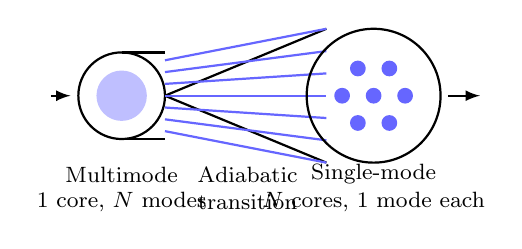
\begin{tikzpicture}[scale=1.0,>=latex]
  % Input face (MM end)
  \draw[thick] (0,0) circle (0.55);
  \fill[blue!25] (0,0) circle (0.32);
  \node[font=\footnotesize] at (0,-1.0) {Multimode};
  \node[font=\footnotesize] at (0,-1.35) {1 core, $N$ modes};
  % Taper body
  \draw[thick] (0.55,0) -- (2.6,0.85);
  \draw[thick] (0.55,0) -- (2.6,-0.85);
  \draw[thick] (0,0.55) .. controls (0.3,0.55) and (0.3,0.55) .. (0.55,0.55);
  \draw[thick] (0,-0.55) .. controls (0.3,-0.55) and (0.3,-0.55) .. (0.55,-0.55);
  % Internal cores (schematic, fanning out)
  \foreach \x/\y in {0.55/0.0, 0.55/0.15, 0.55/-0.15, 0.55/0.30, 0.55/-0.30, 0.55/0.45, 0.55/-0.45} {
    \draw[blue!60,thick] (\x,\y) -- (2.6, 0.85*\y/0.45);
  }
  \node[font=\footnotesize] at (1.6,-1.0) {Adiabatic};
  \node[font=\footnotesize] at (1.6,-1.35) {transition};
  % Output face (SM end)
  \draw[thick] (3.2,0) circle (0.85);
  % 7 cores in hexagonal arrangement
  \foreach \x/\y in {0/0, 0.40/0, 0.20/0.346, -0.20/0.346, -0.40/0, -0.20/-0.346, 0.20/-0.346} {
    \fill[blue!60] (3.2+\x, \y) circle (0.10);
  }
  \node[font=\footnotesize] at (3.2,-1.0) {Single-mode};
  \node[font=\footnotesize] at (3.2,-1.35) {$N$ cores, 1 mode each};
  % Arrows
  \draw[->,thick] (-0.9,0) -- (-0.65,0);
  \draw[->,thick] (4.15,0) -- (4.55,0);
\end{tikzpicture}
\caption{Longitudinal section of a 7-port photonic lantern (schematic, not to scale). The three regions are shown: the multimode input face (one few-mode core), the adiabatic transition (centimetres long), and the single-mode output face ($N$ cores, one mode each). Light travels left to right when the lantern is used as a sensor.}
\label{fig:lantern}
\end{figure}

\subsection{Mode conservation: why the lantern can be lossless}
The central idea is a counting argument. At the SM end, $N$ cores far apart from each other support $N$ guided modes in total, one per core. If the waveguide changes slowly enough along its length (Section~5.4 makes this precise), each guided mode evolves continuously into a guided mode of the next cross-section, and no mode is created or destroyed. The MM end must therefore guide exactly the same number of modes, $N$. Light launched at the MM end in any superposition of its $N$ modes ends up, without loss, in some superposition of the $N$ single-mode cores.

This is a restatement, for waveguides, of the conservation of \'etendue (or brightness, or phase-space volume) in optics. \'Etendue cannot be reduced by a passive system, which is why $N$ modes cannot be squeezed into fewer than $N$ single-mode channels. But nothing forbids distributing $N$ modes over $N$ channels, which is what the lantern does.

The argument also says what goes wrong when the numbers do not match. If the MM end guides more than $N$ modes, light launched into the excess modes has nowhere to go: it is radiated into the cladding during the transition. Going from MM to SM, the excess is lost. If the MM end guides fewer than $N$ modes, light launched backwards from the SM end into some combinations of cores is lost. For a sensor used only from MM to SM this is harmless, but it means some outputs carry less independent information.

By reciprocity, a well-matched lantern works in both directions with low loss, which is why lanterns were first used to pass multimode light through single-mode devices and back~\cite{LeonSaval2005}.

\subsection{Supermode picture: what happens inside the transition}
To understand the transition, freeze the waveguide at a position $z$ and solve the eigenvalue problem of Section~3.1 for that cross-section. The resulting local eigenmodes are called supermodes: profiles $\xi_n(x,y;z)$ with propagation constants $\beta_n(z)$, $n = 1\ldots N$. Follow them from the SM end towards the MM end, using the quantum-well picture of Section~3.2.

\paragraph{Far from the taper (SM end).} The $N$ cores are $N$ identical, well-separated potential wells. Each has one bound state, and all $N$ states have the same energy. The level is $N$-fold degenerate, and any combination of the core modes is an eigenmode.

\paragraph{Cores approaching (tight-binding regime).} As the structure shrinks, the core modes grow relative to the core spacing (the mode-field radius increases as $V$ falls, Section~3.5) and their evanescent tails start to overlap. Light can now tunnel between neighbouring cores, with a coupling rate that grows exponentially as the spacing decreases relative to the mode size. The degeneracy is lifted. The $N$ supermodes become collective modes of the array, exactly like the band of tight-binding states in a crystal of $N$ atoms: the lowest-order supermode has all cores in phase, higher ones have sign changes between cores.

\paragraph{Cores vanishing (multimode end).} Further down the taper, the individual cores become so small ($V \ll 1$) that they hardly perturb the light at all. The supermodes are now guided by the large index step between the fused glass and the low-index capillary, and they become the LP modes of a few-mode step-index guide: $\mathrm{LP}_{01}$, the two $\mathrm{LP}_{11}$, and so on.

Throughout, the supermodes keep their identity and their ordering in effective index. Modes of the same symmetry cannot cross (the ``no-crossing'' rule, or level repulsion), so each supermode at the SM end connects continuously to one LP mode at the MM end. For this mapping to work for all $N$ modes, the arrangement of the cores must have the right symmetry and number: Fontaine~et~al. worked out which core geometries allow every LP mode of the multimode end to evolve into a supermode of the array~\cite{Fontaine2012}. The common hexagonal geometries ($1+6=7$, $1+6+12=19$) and the ring geometries for 3 and 6 cores are examples.

\subsection{The adiabatic condition}
The statement ``each supermode evolves into a supermode'' is the adiabatic theorem of quantum mechanics, with $z$ playing the role of time. Section~10 derives it from the coupled-mode equations; here we state the result and its physical content.

Expand the field on the local supermodes. Because the supermodes themselves change with $z$, power can leak from one to another. The rate of leakage from mode $m$ to mode $n$ is set by the coupling coefficient $\kappa_{nm} = \braket{\xi_n}{\partial_z \xi_m}$, which measures how quickly the shape of mode $m$ changes along $z$, projected onto mode $n$. Leakage is ineffective if the two modes accumulate a large relative phase over the distance on which the coupling acts, because then the contributions from successive slices interfere destructively. The condition for negligible leakage is therefore
\begin{equation}
|\kappa_{nm}(z)| = \left| \braket{\xi_n}{\frac{\partial \xi_m}{\partial z}} \right| \ll |\beta_n(z) - \beta_m(z)|,
\qquad n \neq m.
\label{eq:adiabatic}
\end{equation}
Equivalently: the waveguide must change little over one beat length $2\pi/|\beta_n - \beta_m|$ between any two supermodes. This is the criterion of Love and co-workers for tapered fibres~\cite{Love1991}. When it holds, light launched into supermode $m$ stays in supermode $m$, and only acquires the phase $\int \beta_m\,dz$. The condition must hold everywhere along the taper, not just on average.

\paragraph{Length scales.} With effective-index differences of order $10^{-3}$ between neighbouring supermodes in the middle of the transition, the beat length at $\lambda = \SI{1.55}{\micro\meter}$ is of order \SI{1.5}{\milli\meter} (Section~3.6). The transition must change the structure only slightly over this distance, which leads to transition lengths of centimetres. Where two levels approach, the beat length grows and the criterion becomes harder to meet; for a splitting of $10^{-5}$ the beat length is \SI{15}{\centi\meter}.

\paragraph{The taper profile.} For a fused bundle that is drawn uniformly, every cross-section is a scaled copy of the original, with scale factor $s(z)$ going from 1 at the SM end to the taper ratio at the MM end. The transverse eigenvalue problem then depends on $z$ only through $s$, so the supermodes are functions $\xi_n(x,y;s)$ and the coupling factorises into a geometric part and a rate:
\begin{equation}
\kappa_{nm}(z) = \frac{ds}{dz}\, K_{nm}(s),
\qquad
K_{nm}(s) = \left\langle \xi_n \middle| \frac{\partial \xi_m}{\partial s} \right\rangle.
\label{eq:kappa_scaled}
\end{equation}
The adiabatic criterion becomes $|ds/dz| \ll |\Delta\beta(s)|/|K(s)|$. This says where along the taper the draw can be fast and where it must be slow: slowly where levels are close together or where mode shapes change quickly with scale, quickly elsewhere. Optimised taper profiles exploit this, and it is also a strong simplification for simulation (Section~10.4).

\subsection{The single-mode end: degeneracy and freezing}
The adiabatic criterion necessarily fails near the SM end, where the $N$ levels merge into a degenerate one and $\Delta\beta \to 0$. This sounds alarming but is mostly harmless. Near the SM end the cores are also decoupling: tunnelling between them falls exponentially as they separate, and soon the power in each core stops changing. The evolution ``freezes''. Whatever happens among nearly degenerate supermodes just before freezing only determines how the light is finally distributed over the cores, not whether it is lost.

The practical consequence is that the final mapping from input modes to output cores is very sensitive to the details of the last part of the transition: small differences between the cores, small asymmetries of the draw, residual stress. Two lanterns made to the same design can have quite different mappings, and this is why every lantern must be calibrated individually.

A lantern can be deliberately made \emph{mode-selective} by using dissimilar cores, so that the SM-end levels are not degenerate~\cite{LeonSaval2014}. Then the adiabatic theorem holds all the way, and each LP mode of the MM end maps onto one specific core. As shown in Section~6.3, this is exactly the wrong property for a wavefront sensor.

\subsection{The transfer matrix}
Putting the pieces together: the lantern is a linear, passive device acting on $N$ complex input amplitudes (the projections $u_n$ of the incident field on the LP modes of the MM end) and producing $N$ complex output amplitudes (the amplitudes $v_k$ of the fundamental modes of the $N$ single-mode cores). It is therefore described by an $N \times N$ complex matrix $A$, the \emph{transfer matrix}:
\begin{equation}
\vvec = A\, \uvec,
\qquad
v_k = \sum_{n=1}^{N} A_{kn}\, u_n.
\label{eq:transfer}
\end{equation}
The column $n$ of $A$ is the output produced by launching LP mode $n$ alone at the input. Its main properties are the following.
\begin{itemize}
\item \textbf{Unitarity.} For an ideal, lossless lantern, $A$ is unitary, $A^\dagger A = 1$, so total power is conserved: $\sum |v_k|^2 = \sum |u_n|^2$. This unitarity refers to the guided-mode subspace only. Real devices have some loss, which shows up as singular values of $A$ slightly below 1; radiation losses during the transition are not captured by the $N \times N$ matrix.
\item \textbf{Density.} In a standard lantern, each column of $A$ is spread over many cores with comparable magnitudes and definite phases: each input mode illuminates many outputs. In a mode-selective lantern, $A$ is close to a permutation matrix times a diagonal matrix of phases.
\item \textbf{Reciprocity.} Light sent backwards from the cores to the MM end is described by the transpose of $A$ (not its inverse), in the appropriate mode basis: $A^T$, not $A^{-1}$.
\item \textbf{Sensitivity.} $A$ depends on wavelength, on temperature, and on the exact geometry. It cannot be reliably predicted from the nominal design to the accuracy needed for wavefront sensing, which is why it is measured, or rather why the sensor response is measured directly (Section~7.1).
\end{itemize}
The matrix $A$ is the single object that a lantern simulation must deliver (Section~8).

\subsection{Chromatic behaviour}
The transfer matrix depends on wavelength for two reasons. First, the phases accumulated along the transition, $\int \beta_n\,dz$, depend on wavelength, and so do the differences between them, which control how modes interfere at the output. Roughly, if the transition contains $L/L_B$ beat lengths between two supermodes, a relative change of wavelength $\Delta\lambda/\lambda$ changes their relative phase by about $2\pi (L/L_B)(\Delta\lambda/\lambda)$. $A$ changes appreciably when this approaches $\pi$, so a transition containing tens of beat lengths decorrelates over a bandwidth of a few percent. This is an order-of-magnitude estimate, but it explains why the response of a lantern varies strongly across a broad band. Second, the mode count of the MM end depends on $V \propto 1/\lambda$ (Section~3.4), so a lantern matched at one wavelength is over- or under-moded at another.

Chromaticity is a nuisance in broadband light, where the response averages over wavelengths and partly washes out. It becomes an asset if the outputs are spectrally dispersed: each spectral channel then gives an independent set of $N$ fluxes, multiplying the number of measurements~\cite{Lin2025}.

\subsection{Polarisation}
In the weakly guiding approximation, the lantern acts identically on both polarisations, so $A$ is the same for each and unpolarised detection simply adds two identical patterns. Real lanterns have small birefringence from stress and from non-circular cores, so the two polarisations see slightly different transfer matrices. Separating the polarisations at the output can then double the number of independent measurements~\cite{Lin2023PRL}.

%========================================================
\section{The lantern as a wavefront sensor}
\label{sec:sensor}
%========================================================

\subsection{The forward model}
We now have every ingredient needed to write the complete measurement model (Figure~\ref{fig:chain}).
\begin{enumerate}
\item \textbf{Pupil.} The field in the pupil is $P(x,y)\exp[i\varphi(x,y)]$, with $\varphi$ the residual wavefront phase in radians.
\item \textbf{Focal plane.} The telescope forms $E = \mathcal{F}[P e^{i\varphi}]$ on the input face of the lantern (Section~2.3).
\item \textbf{Projection.} Only the guided part of $E$ enters. Projecting on the $N$ LP modes of the MM end gives the vector of modal amplitudes, $u_n = \braket{\psi_n}{E}$ (Section~4.1).
\item \textbf{Lantern.} The transition multiplies $\uvec$ by the transfer matrix: $\vvec = A\uvec$ (Section~5.6).
\item \textbf{Detection.} A detector measures the power in each output core, $p_k = |v_k|^2$.
\end{enumerate}

Combining the steps gives the sensor model in one line:
\begin{equation}
p_k(\varphi) = \left| \sum_{n=1}^{N} A_{kn}\, \braket{\psi_n}{\mathcal{F}[P e^{i\varphi}]} \right|^2,
\qquad k = 1,\ldots,N.
\label{eq:forward}
\end{equation}
In a real instrument the measured signal is this quantity multiplied by the number of photons collected in the exposure, plus photon noise, detector noise and background. If the outputs are dispersed, the model is evaluated separately at each wavelength with the corresponding $A(\lambda)$.

Note the structure: a nonlinear but simple map from $\varphi$ to $\uvec$ (through the exponential only), a linear unitary map from $\uvec$ to $\vvec$, and a quadratic detection. All the specific physics of the device is concentrated in $A$.

\begin{figure}[t]
\centering
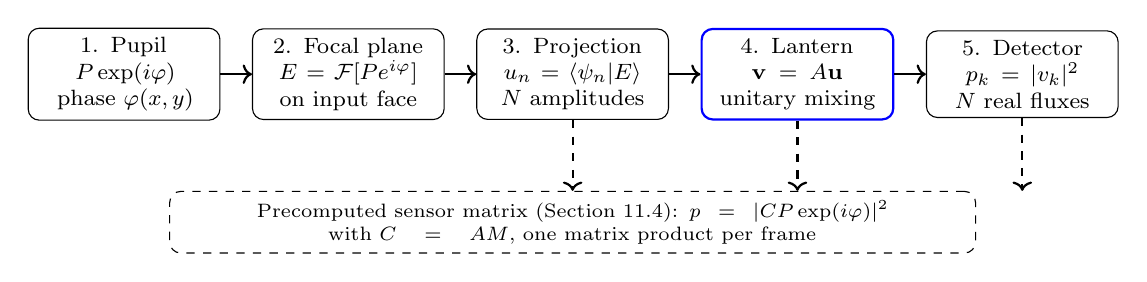
\begin{tikzpicture}[
  node distance=0.4cm,
  box/.style={draw,rounded corners,align=center,minimum height=1.1cm,text width=2.2cm,font=\footnotesize},
  arrow/.style={->,thick}
]
\node[box] (pupil) {1. Pupil\\$P\exp(i\varphi)$\\phase $\varphi(x,y)$};
\node[box,right=of pupil] (focal) {2. Focal plane\\$E=\mathcal{F}[P e^{i\varphi}]$\\on input face};
\node[box,right=of focal] (proj) {3. Projection\\$u_n=\braket{\psi_n}{E}$\\$N$ amplitudes};
\node[box,right=of proj,draw=blue,thick] (lantern) {4. Lantern\\$\vvec=A\uvec$\\unitary mixing};
\node[box,right=of lantern] (det) {5. Detector\\$p_k=|v_k|^2$\\$N$ real fluxes};
\draw[arrow] (pupil) -- (focal);
\draw[arrow] (focal) -- (proj);
\draw[arrow] (proj) -- (lantern);
\draw[arrow] (lantern) -- (det);
\node[below=0.9cm of proj,draw,dashed,rounded corners,align=center,font=\scriptsize,text width=10cm] (precomp) {Precomputed sensor matrix (Section~11.4): $p=|C P\exp(i\varphi)|^2$ with $C=AM$, one matrix product per frame};
\draw[arrow,dashed] (proj.south) -- (proj.south |- precomp.north);
\draw[arrow,dashed] (lantern.south) -- (lantern.south |- precomp.north);
\draw[arrow,dashed] (det.south) -- (det.south |- precomp.north);
\end{tikzpicture}
\caption{The five steps of the forward model of Section~6.1. The map from $\varphi$ to $\uvec$ is nonlinear only through the exponential; the lantern step is a fixed unitary matrix; detection is quadratic. Because the Fourier transform is unitary, steps 2 to 4 collapse into a single precomputed matrix for simulation (Section~11.4).}
\label{fig:chain}
\end{figure}

\subsection{Each output is an interferometer}
Expand the modulus squared:
\begin{equation}
p_k = \sum_n |A_{kn}|^2 |u_n|^2 + 2\sum_{n<n'} \mathrm{Re}\!\left[ A_{kn} A_{kn'}^*\, u_n u_{n'}^* \right].
\label{eq:interferometer}
\end{equation}
The first sum depends only on the powers in the modes. The second sum is a set of interference terms: each pair of input modes $(n,n')$ contributes a fringe whose value depends on the relative phase of the modal amplitudes, $\arg u_n - \arg u_{n'}$, shifted by a fixed, device-specific phase, $\arg A_{kn} - \arg A_{kn'}$. Each output port is therefore a multi-beam interferometer with $N$ arms whose weights and phase offsets are set, once and for all, by the fabrication of the lantern. The $N$ ports are $N$ such interferometers with different offsets.

This is the essential point of the whole tutorial. A detector cannot measure phase directly, but an interferometer converts relative phase into intensity. The lantern is a passive, compact, common-path $N$-port interferometer acting on the modes of the focal-plane field.

In matrix language, $p_k = \uvec^\dagger M_k \uvec$ with $M_k = \mathbf{a}_k \mathbf{a}_k^\dagger$, where $\mathbf{a}_k$ is the complex conjugate of row $k$ of $A$. Each $M_k$ is a rank-one Hermitian matrix. For a unitary $A$, $\sum_k M_k = A^\dagger A = 1$, so $\sum_k p_k = \sum_n |u_n|^2$, the total guided power.

\subsection{The linear response, derived}
\label{sec:sign}
Write the aberration as $\varphi = \sum_m a_m Z_m$ and expand to first order in the coefficients $a_m$. Since $e^{i\varphi} \approx 1 + i\varphi$, the modal amplitudes become
\begin{equation}
u_n \approx u_{0,n} + i \sum_m a_m\, w_{nm},
\qquad
u_{0,n} = \braket{\psi_n}{\mathcal{F}[P]},
\qquad
w_{nm} = \braket{\psi_n}{\mathcal{F}[P Z_m]}.
\label{eq:linear_u}
\end{equation}
Here $\uvec_0$ is the modal content of the unaberrated PSF, and $w_{nm}$ is the amount of mode $n$ excited by a unit amount of aberration $m$. Let $\vvec_0 = A\uvec_0$ be the unaberrated output amplitudes. Then $\vvec = \vvec_0 + i\sum_m a_m A \mathbf{w}_m$, and expanding $|v_k|^2$ to first order gives the flux response
\begin{equation}
p_k \approx p_{0,k} + \sum_m B_{km}\, a_m,
\qquad
B_{km} = -2\,\mathrm{Im}\!\left[ \mathbf{v}_0^* (A\mathbf{w}_m)_k \right] = -2\sum_{n,n'} \mathrm{Im}\!\left[ A_{kn}^* A_{kn'}\, u_{0,n}^*\, w_{n'm} \right].
\label{eq:linear_p}
\end{equation}
$B$ is the interaction matrix of the sensor, the same object used for every AO wavefront sensor. To see what it requires of the lantern, use symmetry. Assume, as is usual, that the pupil $P$ is real and centrally symmetric, that the PSF is centred on the axis of the lantern, and that the LP modes are chosen real, in their cos and sin forms. Each $\mathrm{LP}_{lm}$ mode then has a definite parity $(-1)^l$ under inversion through the centre, and each Zernike has a definite parity too (Section~2.4). The Fourier transform preserves parity, maps real even functions to real functions and real odd functions to imaginary functions. It follows that:
\begin{itemize}
\item $\uvec_0$ is real, and non-zero only on even modes ($l$ even), because the unaberrated PSF is even;
\item for an \textbf{even} aberration, $\mathbf{w}_m$ is real and non-zero only on even modes;
\item for an \textbf{odd} aberration, $\mathbf{w}_m$ is purely imaginary and non-zero only on odd modes.
\end{itemize}
Substituting into the expression for $B$ gives two conditions:
\begin{align}
\text{even } Z_m:\quad
B_{km} &= -2 \sum_{n,n'\ \mathrm{even}} \mathrm{Im}\!\left[ A_{kn}^* A_{kn'} \right] u_{0,n}\, w_{n'm},
\label{eq:B_even}\\
\text{odd } Z_m:\quad
B_{km} &= -2 \sum_{n\ \mathrm{even},\, n'\ \mathrm{odd}} \mathrm{Re}\!\left[ A_{kn}^* A_{kn'} \right] u_{0,n}\, c_{n'm},
\qquad w_{n'm} = i\, c_{n'm}.
\label{eq:B_odd}
\end{align}
These two formulas explain everything about the sign problem.

\paragraph{A plain camera.} A pixel at position $\xi$ records $|E(\xi)|^2$ with $E(\xi) = \sum_n \psi_n(\xi) u_n$ (plus the unguided part). It is a ``lantern'' whose row $k$ is $\psi_n(\xi_k)$, a set of real numbers. Then $\mathrm{Im}[A_{kn}^* A_{kn'}] = 0$ for every pair, and even aberrations produce no first-order signal: this is the sign ambiguity of Section~1.2. Odd aberrations do produce a signal, because off-centre pixels mix even and odd modes with real weights.

\paragraph{A modal power meter, or a mode-selective lantern.} If each output receives a single input mode ($A$ diagonal up to a permutation and phases), each row has only one non-zero entry. Both sums vanish: such a device is blind at first order to every aberration, even and odd. Physically, the power in any single mode changes only quadratically with a small aberration of a centred PSF (as for the single-mode fibre in Section~4.3).

\paragraph{A standard lantern.} Its rows mix even and odd modes, so odd aberrations are sensed; and the entries of a row have non-trivial relative phases, so $\mathrm{Im}[A_{kn}^* A_{kn'}] \neq 0$ and even aberrations are sensed too, with their sign. The lantern's ``defect'', that it scrambles the modes with uncontrolled phases, is exactly the property that makes it a wavefront sensor. This analysis is in the spirit of the theoretical framework of Lin~et~al.~\cite{Lin2022}, which derives linear and higher-order reconstruction models and performance metrics; the companion paper by Lin and Fitzgerald characterises few-port lanterns numerically and discusses how their response can be optimised~\cite{Lin2023}.

\subsection{How many modes can be sensed}
The interaction matrix has $N$ rows, so its rank is at most $N$: a lantern with $N$ ports senses at most $N$ modes linearly per wavelength channel and polarisation~\cite{Lin2023PRL}. Under the idealisations of Section~\ref{sec:sign} (lossless lantern, centred PSF, symmetric pupil), one more constraint applies. Summing the rows of $B$ gives the first-order change of the total guided power $\sum |u_n|^2$, which vanishes by the same symmetry argument (the coupled power changes only at second order). The rows of $B$ then sum to zero and the rank is at most $N-1$. In practice, losses, asymmetries and an off-centre PSF relax this constraint, and the useful number of modes is set by the conditioning of $B$, i.e.\ by how its singular values compare with the noise.

Two ways to get more measurements than $N$ per exposure are to disperse the outputs, so that each of several spectral channels gives its own $N$ fluxes with a different $A(\lambda)$~\cite{Lin2025}, and to separate the two polarisations of a birefringent lantern~\cite{Lin2023PRL}.

\subsection{Noise and sensitivity}
Let $N_{\rm ph}$ be the number of photons collected in one exposure, so that the expected counts are $N_{\rm ph} p_k$ (with $p$ normalised to the input power). In the photon-noise limit, the counts in different ports are independent Poisson variables with variances $N_{\rm ph} p_{0,k}$. A linear reconstructor $\hat{\mathbf{a}} = R(\pvec - \pvec_0)$ (Section~7.2) then has an error covariance given by standard error propagation, with $B$ expressed per unit input power:
\begin{equation}
\mathrm{cov}[\hat{\mathbf{a}}] = \frac{1}{N_{\rm ph}}\, R\, \mathrm{diag}(\pvec_0)\, R^T,
\qquad
R = B^+.
\label{eq:cov}
\end{equation}
The error on each mode falls as $1/\sqrt{N_{\rm ph}}$, and the prefactor, a property of $B$ and $\pvec_0$, measures the intrinsic sensitivity of the sensor to that mode. Guyon~\cite{Guyon2005} showed that sensors working in or near the focal plane can be much more sensitive to low-order modes than a Shack--Hartmann sensor, because they exploit the full aperture as an interferometer baseline. The lantern belongs to this family. Three practical points add to its photon efficiency: no light is diverted to a separate sensing arm, since the measured photons are the science photons; the PSF core, where most photons are, is exactly where the lantern samples; and only $N$ pixels per spectral channel are read, which keeps detector read noise small.

\subsection{Linear range and nonlinearity}
Every flux is bounded between 0 and the total guided power, and the interference terms of Section~6.2 vary as the cosine of a relative phase. The response to a growing aberration is therefore roughly sinusoidal: linear near zero, then saturating, then folding back. The linear range corresponds to modal phase differences well below a radian, i.e.\ residual wavefronts of a fraction of a radian rms. Beyond it, a linear reconstructor underestimates the aberration; further out, different aberrations can produce the same fluxes and the sign of the correction can be wrong. Lin~et~al.\ report stable closed-loop operation on the SCExAO testbed up to about \SI{400}{\nano\meter} of low-order Zernike error~\cite{Lin2023PRL}. Because the coupled power also falls as the aberration grows (Section~4.3), large errors are additionally penalised by a loss of signal.

The practical conclusion is that the lantern needs to be preceded by an AO system that brings the residuals into its linear range. Nonlinear reconstructors (Section~7.3) extend the range but do not change this conclusion fundamentally.

\subsection{Petal modes}
A petal mode is a piston on one pupil island. On a pupil with a symmetric set of spiders, any such pattern can be split into a part that is even and a part that is odd under inversion. Both parts change the focal-plane field strongly near the PSF core, and therefore excite the low-order LP modes with large $w$ coefficients. By the analysis of Section~\ref{sec:sign}, a standard lantern responds linearly to both. This is the formal reason for its sensitivity to petal modes, which slope-based pupil sensors see only weakly (and in practice only through finite-width spider diffraction), and it has been demonstrated on the SCExAO testbed, where the lantern sensor corrected petal modes in closed loop~\cite{Lin2023PRL}.

%========================================================
\section{Calibration, reconstruction and experiments}
%========================================================

\subsection{Calibration}
Because $A$ cannot be predicted accurately (Section~5.5), a lantern sensor is calibrated empirically, exactly like a pupil-plane sensor. The procedure uses the deformable mirror as a source of known aberrations.
\begin{enumerate}
\item \textbf{Reference.} With the best available wavefront (for instance, after the first-stage AO has converged on an internal source), record the fluxes $\pvec_0$.
\item \textbf{Push-pull.} For each mode $m$, apply $+\delta Z_m$ on the DM, record the fluxes, apply $-\delta Z_m$, record again. The centred difference removes the second-order term of the response and gives one column of the interaction matrix:
\begin{equation}
B_{\cdot m} \approx \frac{\pvec(+\delta Z_m) - \pvec(-\delta Z_m)}{2\delta}.
\label{eq:pushpull}
\end{equation}
\item \textbf{Choice of amplitude.} $\delta$ must be small enough to stay in the linear regime of Section~6.6 and large enough to rise above noise and drifts. Several push-pull cycles are usually averaged.
\item \textbf{Normalisation.} Dividing each flux vector by its sum, $\bar{\pvec} = \pvec/\sum_k p_k$, removes fluctuations of the source brightness (seeing, scintillation, clouds). It also removes one degree of freedom, consistent with the rank argument of Section~6.4.
\end{enumerate}
The interaction matrix depends on everything upstream and downstream of the lantern: the pupil, the focal ratio, the centring of the PSF on the fibre, the wavelength band, the temperature of the lantern. It drifts slowly and must be re-measured. The reference $\pvec_0$ is particularly important, because it defines the wavefront to which the loop converges: any error in the reference becomes a static aberration in the corrected wavefront. A common choice is to define $\pvec_0$ as the fluxes at the wavefront that maximises a science metric, such as the coupling into the fibres or the contrast in a coronagraphic image.

\subsection{Linear reconstruction and closed loop}
The linear reconstructor is the pseudo-inverse of $B$, computed by singular value decomposition, $B = U\Sigma V^T$:
\begin{equation}
\hat{\mathbf{a}} = R\,(\pvec - \pvec_0),
\qquad
R = V\Sigma^+ U^T.
\label{eq:reconstructor}
\end{equation}
In $\Sigma^+$, singular values below a threshold are set to zero rather than inverted, to avoid amplifying noise along poorly sensed directions. The number of retained singular values is the number of modes actually controlled, which is the practical answer to the question of Section~6.4.

In closed loop the lantern measures the residual wavefront after the DM, and the DM command $\mathbf{c}$ is updated by an integrator with gain $g$, often with a small leak $\ell$ to keep the commands bounded:
\begin{equation}
\mathbf{c}_{t+1} = (1-\ell)\,\mathbf{c}_t - g\, R\,(\pvec_t - \pvec_0).
\label{eq:integrator}
\end{equation}
Because the reconstructor is only valid near $\pvec_0$, the loop must be closed starting from a wavefront already inside the linear range, which in practice means after the first-stage AO is running.

\subsection{Beyond the linear regime}
Several strategies extend the range or the number of sensed modes.
\begin{itemize}
\item \textbf{Second-order models.} Expanding the response to second order, $p_k = p_{0,k} + \sum_m B_{km} a_m + \frac{1}{2}\sum_{m,m'} H_{k,mm'} a_m a_{m'}$, and solving iteratively (for example by Gauss--Newton) captures the curvature of the response. The second-order coefficients can be measured with additional DM pokes or computed from a model of $A$. Quadratic reconstructors for lanterns are analysed in~\cite{Lin2022,Lin2023}.
\item \textbf{Model-based phase retrieval.} If $A$ is known, from a fit to calibration data or from simulation, the full forward model of Section~6.1 can be fitted directly to the measured fluxes. This is the most general approach and the one that benefits most from accurate simulation.
\item \textbf{Neural networks.} A network trained on many pairs of known aberrations and measured fluxes learns the inverse map, including its nonlinear part. Norris~et~al.\ used this approach with a 19-output lantern in the laboratory~\cite{Norris2020}. Networks trade physical transparency for flexibility and must be retrained when the device or the optical setup changes.
\item \textbf{Spectral dispersion.} Dispersing the outputs gives $N$ fluxes per spectral channel, each set with a different $A(\lambda)$. This adds independent measurements, improves conditioning, and helps lift ambiguities in the nonlinear regime~\cite{Lin2025}.
\item \textbf{Pre- and post-lantern optics.} Phase masks in front of the lantern, or interferometric recombination of its outputs, can tailor the response; Lin~et~al.\ consider such optimisations~\cite{Lin2023}.
\end{itemize}

\subsection{Experimental record}
\begin{table}[h]
\centering
\caption{Experimental demonstrations of the photonic-lantern wavefront sensor.}
\label{tab:experiments}
\small
\begin{tabular}{@{}llp{7cm}@{}}
\toprule
Year & Reference & Result \\
\midrule
2025 & Lin~et~al.~\cite{Lin2025} & Spectral dispersion of the lantern outputs improves correction; first on-sky real-time wavefront control with a lantern sensor. \\
2023 & Lin~et~al.~\cite{Lin2023PRL} & Real-time closed loop on the Subaru/SCExAO testbed; stable up to about \SI{400}{\nano\meter} of low-order Zernike error; petal modes corrected; about $10\times$ rejection at \SI{1}{\second} timescales for about \SI{30}{\nano\meter} rms of injected low-order error. \\
2020 & Norris~et~al.~\cite{Norris2020} & 19-output lantern; neural-network reconstruction of low-order aberrations; established the focal-plane lantern sensor concept. \\
2018 & Corrigan~et~al.~\cite{Corrigan2018} & Laboratory AO testbed; low-order wavefront sensing with a photonic lantern. \\
\bottomrule
\end{tabular}
\end{table}
The results from the SCExAO testbed were obtained with a 19-port lantern behind the facility and extreme AO of the Subaru telescope~\cite{Lin2023PRL,Lin2025}. They show the sensor working as intended: as a second stage, correcting low-order and petal residuals of a few tens of nanometres.

\subsection{Comparison with other wavefront sensors}
\begin{table}[h]
\centering
\caption{Comparison of wavefront-sensor families.}
\label{tab:compare}
\small
\begin{tabular}{@{}lcccc@{}}
\toprule
Property & Shack--Hartmann & Pyramid & Focal-plane image & Photonic lantern \\
\midrule
Location & Pupil (separate arm) & Near focal plane (separate arm) & Science focal plane & Science focal plane \\
Common path with science & No & No & Yes & Yes \\
Measures & Local slopes & Slopes to phase, depending on modulation & Intensity image & $N$ mode-mixed fluxes \\
Number of modes & High & High & High, with diversity & About $N$ per channel \\
Even modes, first order & Yes & Yes & No, needs diversity & Yes \\
Petal modes & Weak & Better than SH & Strong & Strong \\
Linear range & Large & Adjustable with modulation & Small & Small, below a radian \\
Photons for sensing & Diverted & Diverted & Science photons & Science photons, also fed to a spectrograph \\
\bottomrule
\end{tabular}
\end{table}
Table~\ref{tab:compare} makes the complementary role clear. Pupil-plane sensors are the right first stage: many modes, large range, robust. A lantern adds a common-path, photon-efficient, petal-sensitive second stage for a few low-order modes, located exactly where the science light is coupled into single-mode fibres.

%========================================================
\section{Simulating a lantern I: goals and idealised models}
%========================================================

\subsection{What a simulation must deliver}
The sensor model of Section~6.1 separates cleanly into a telescope part (pupil, Fourier transform, projection onto the LP modes) and a device part (the transfer matrix $A$). The telescope part is standard Fourier optics. The device part requires solving for light propagation through a three-dimensional, slowly varying dielectric structure. Its output, the thing a lantern simulation must deliver, is the transfer matrix as a function of wavelength, $A(\lambda)$, defined with respect to two fixed mode bases:
\begin{itemize}
\item at the input, the $N$ guided modes $\psi_n$ of the multimode section;
\item at the output, the fundamental modes of the $N$ single-mode cores.
\end{itemize}
The column $n$ of $A$ is obtained by launching $\psi_n$ alone at the input, propagating to the output, and projecting the output field on each core mode. Any light not captured by the $N$ core modes is loss, and shows up as $A^\dagger A < 1$.

Two conventions matter when comparing simulations with each other or with experiment.
\begin{itemize}
\item \textbf{Phase conventions of the bases.} Each mode is defined only up to a sign (for real modes) or a phase. Changing the phase of input mode $n$ multiplies column $n$ of $A$ by that phase; changing the phase of output core $k$ multiplies row $k$. Since the detector measures $|v_k|^2$, the row phases have no observable effect, so $A$ is physically meaningful only up to a diagonal matrix of phases on the left. The column phases must be fixed consistently with the convention used to compute $\uvec$.
\item \textbf{Degenerate pairs.} The $\mathrm{LP}_{lm}$ modes with $l \geq 1$ come in degenerate pairs, and any rotation of a pair is equally valid. The orientation used to define the modes in the lantern simulation must match the one used in the telescope part of the model.
\end{itemize}
A simulation is useful for three purposes: to design a lantern (choose core layout, taper ratio, taper profile and length for a target response); to understand and predict trends (chromatic behaviour, tolerance to fabrication errors); and to provide realistic transfer matrices for end-to-end AO simulations before a device exists.

\subsection{Why full-wave methods are impractical}
The most general approach would be to solve Maxwell's equations directly, for example with the finite-difference time-domain (FDTD) method. A simple count shows why this is impractical. Take a transverse domain of \SI{100}{\micro\meter} $\times$ \SI{100}{\micro\meter} and a transition length of \SI{3}{\centi\meter} at $\lambda = \SI{1.55}{\micro\meter}$ in glass of index 1.45, where the wavelength is about \SI{1.07}{\micro\meter}. A grid fine enough to resolve the wavelength, with about ten points per wavelength, needs about $1000 \times 1000 \times 300000 \approx 3\times 10^{11}$ cells, each with six field components, and the time stepping must cover the transit time of light through the whole device. This is far beyond routine computing, and would have to be repeated for each input mode and each wavelength.

The structure of the problem suggests better approaches, and both exploit the same physical fact: the field travels essentially in one direction, and varies slowly along it.

The paraxial approximation (Section~2.2) removes the fast carrier $\exp(ik_0 n_0 z)$ and turns the problem into a two-dimensional evolution equation in $z$. This is the basis of the beam propagation method (Section~9). The guided-mode structure means that, at every $z$, the light lives in an $N$-dimensional space of local eigenmodes. Evolving $N$ amplitudes instead of a full field is the basis of coupled-mode theory (Section~10).

A third family, eigenmode expansion (EME), approximates the structure as a stack of short, uniform sections, expands the field on the modes of each section, and matches fields at the interfaces. It is closely related to coupled-mode theory and is the discrete-step version of it.

\begin{table}[h]
\centering
\caption{Comparison of simulation methods.}
\label{tab:methods}
\small
\begin{tabular}{@{}lllll@{}}
\toprule
Method & Unknowns & Cost per launch & Captures radiation loss & Typical use \\
\midrule
Idealised modal model & none & negligible & no & reconstructors, statistics \\
Beam propagation & field on 2-D grid, $10^5$--$10^6$ points & high: thousands of $z$ steps & yes & reference solutions, arbitrary geometry \\
Coupled-mode theory & $N$ amplitudes & low after eigenmode setup & no (guided modes only) & design sweeps, many wavelengths \\
\bottomrule
\end{tabular}
\end{table}

\subsection{Idealised models}
Many questions about the sensor do not depend on the details of a particular lantern: how a reconstructor behaves, how noise propagates, how many modes can be controlled for a given $N$, how the performance varies across a population of devices. For these, it is enough to compute the LP modes of the input face (Section~3.3) and to choose $A$ by hand.

\paragraph{Random unitary matrices.} A standard lantern scrambles the modes with phases that are effectively random. A natural model is therefore a unitary matrix drawn uniformly from the unitary group, the Haar measure. A correct and simple recipe~\cite{Mezzadri2007}: draw an $N\times N$ matrix $Z$ of independent complex Gaussian entries; compute its QR decomposition $Z = QR$; and multiply each column $j$ of $Q$ by the phase of the diagonal element $R_{jj}$, i.e.\ by $R_{jj}/|R_{jj}|$. The last step is necessary; without it the distribution is not uniform. Averaging results over many such matrices gives the expected performance of a ``typical'' lantern and its spread.

\paragraph{Structured matrices.} To study a specific idea, $A$ can be built from a hypothesis: for example, a mode-selective lantern ($A$ close to a permutation times phases), which, by Section~\ref{sec:sign}, should show no first-order response; or a lantern whose supermodes map onto core patterns of known symmetry.

\paragraph{Measured matrices.} A transfer matrix can be estimated from laboratory data, for example by fitting the forward model of Section~6.1 to the fluxes measured for a set of known DM aberrations. The fit determines $A$ up to the unobservable row phases. Such an empirical $A$ turns a laboratory characterisation into a simulation model.

\subsection{The input modes in practice}
In every model, the projection $u_n = \braket{\psi_n}{E}$ requires the modes of the multimode section, sampled on the same grid as the focal field. For an ideal step-index multimode section they follow from the characteristic equation of Section~3.3, solved numerically for $U$ at each $l$, with the field profiles built from Bessel functions. If the multimode section is not an ideal circular step-index guide (for example, a fused bundle whose outer boundary is not perfectly round, or which retains a residual index structure from the original cores), its modes must be computed numerically, by a finite-element or finite-difference eigenmode solver applied to the actual cross-section. This is the same computation that coupled-mode theory performs along the taper (Section~10).

Two sampling requirements follow. The focal field must be sampled finely enough to resolve the highest-order mode, a few points per lobe at least. And the scaling between the focal plane and the lantern face, set by the focal ratio $F$, must be chosen to optimise the overlap between the PSF and the guided modes; this is a design parameter of the instrument and is usually found by maximising the total coupling $\eta_{\rm tot}$ for the expected residual wavefronts.

%========================================================
\section{Simulating a lantern II: the beam propagation method}
%========================================================

The beam propagation method (BPM) solves the paraxial wave equation of Section~2.2 as an initial-value problem: given the field on the input face, march it step by step in $z$ through the actual index distribution $n(x,y,z)$ of the lantern. It makes no assumption about which modes exist, so it captures non-adiabatic coupling, radiation loss and arbitrary geometries. It is the reference method against which faster approaches are checked. Textbook treatments of waveguide modes and of the BPM are given in~\cite{SnyderLove,Okamoto2006}.

\subsection{The equation and its validity}
We solve the paraxial equation in operator form, with $H$ a Hermitian operator on functions of $(x,y)$:
\begin{equation}
\frac{\partial u}{\partial z} = i\, H(z)\, u,
\qquad
H(z) = \underbrace{\frac{\nabla_\perp^2}{2 k_0 n_0}}_{D} + \underbrace{\frac{k_0\left(n^2 - n_0^2\right)}{2 n_0}}_{V}.
\label{eq:bpm_op}
\end{equation}
$D$ describes diffraction, $V$ describes the refraction by the local index. Because $H$ is Hermitian, the exact evolution is unitary and conserves $\int |u|^2\,dx\,dy$, except for power that leaves through the boundaries of the computational domain.

The paraxial approximation requires that the light travels at small angles to the $z$ axis. Guided light in a fibre travels at angles of order $\mathrm{NA}/n$, a few degrees for lanterns, so the approximation is excellent for the guided field. The reference index $n_0$ should be chosen close to the effective indices of the guided modes, typically between $n_2$ and $n_1$, so that the envelope $u$ varies slowly and the phase errors of the paraxial approximation stay small. When higher angles matter, wide-angle formulations based on Pad\'e approximants of the square-root operator improve on the paraxial equation at modest extra cost~\cite{Hadley1992}.

\subsection{Split-step Fourier BPM}
The exact solution over a step $\Delta z$ is $u(z + \Delta z) = \exp(i\Delta z\,H)u(z)$, if $H$ is treated as constant over the step. $D$ and $V$ do not commute, so the exponential cannot simply be split into a product. The symmetric (Strang) splitting does so with an error of order $\Delta z^3$ per step, $\Delta z^2$ overall:
\begin{equation}
u(z + \Delta z) \approx e^{\,i\frac{\Delta z}{2}D}\;
e^{\,i\Delta z\, V(z + \Delta z/2)}\;
e^{\,i\frac{\Delta z}{2}D}\; u(z).
\label{eq:strang}
\end{equation}
Each factor is easy to apply in the right space. The diffraction operator is diagonal in Fourier space, where it multiplies each plane-wave component by a phase; the refraction operator is diagonal in real space, where it multiplies the field by a phase screen:
\begin{align}
e^{\,i\frac{\Delta z}{2}D}:\;
\tilde{u}(k_x,k_y) &\mapsto \tilde{u}(k_x,k_y)\,
\exp\!\left[-i\,\frac{\Delta z}{2}\,
\frac{k_x^2 + k_y^2}{2 k_0 n_0}\right],
\label{eq:diffraction_step}\\
e^{\,i\Delta z\, V}:\;
u(x,y) &\mapsto u(x,y)\, e^{\,i\Delta z\, V(x,y)}.
\label{eq:refraction_step}
\end{align}
One step therefore costs two FFTs and a few pointwise multiplications. This scheme was introduced by Feit and Fleck for graded-index fibres~\cite{FeitFleck1978}, and it is the same algorithm used in quantum mechanics (the split-operator method) and in atmospheric optics (phase screens separated by Fresnel propagation). Its strengths are spectral accuracy in the transverse direction and simplicity. Its weaknesses for lanterns are that the grid is uniform, so it must resolve the smallest feature everywhere, and periodic, so light leaving one side re-enters on the other unless absorbed.

\subsection{Finite-difference BPM}
The alternative discretises the transverse Laplacian with finite differences, which turns $H$ into a large sparse matrix, and advances in $z$ with the Crank--Nicolson scheme:
\begin{equation}
\left( 1 - \frac{i\Delta z}{2} H_{j+1/2} \right) u^{j+1} = \left( 1 + \frac{i\Delta z}{2} H_{j+1/2} \right) u^{j}.
\label{eq:crank}
\end{equation}
This is the Cayley form of the exponential, $(1 - i\Delta z H/2)^{-1}(1 + i\Delta z H/2)$, which is exactly unitary when $H$ is Hermitian. The scheme is therefore unconditionally stable and conserves power, and it is second-order accurate in $\Delta z$. Each step requires solving a sparse linear system. In two transverse dimensions this is done efficiently by the alternating-direction implicit (ADI) method of Peaceman and Rachford, which splits the step into two half-steps, implicit in $x$ and then in $y$; each half-step is a set of independent tridiagonal systems, solved in time proportional to the number of grid points.

The main advantage of finite differences for lanterns is freedom in the grid. Non-uniform grids, fine where the cores are and coarse in the cladding, are straightforward~\cite{Shibayama1999}. Adaptive grids, which refine automatically where the field varies quickly and follow the cores as the structure shrinks, reduce the cost further; the open-source code \texttt{lightbeam} implements a finite-difference BPM with a transverse adaptive mesh~\cite{lightbeam}. One caution: the Cayley form maps very large eigenvalues of $H$ to a phase close to $-1$ rather than damping them, so high spatial frequencies are propagated inaccurately if $\Delta z$ is too large. The step must remain small compared with the diffraction length of the finest grid features that carry power.

\subsection{Boundaries}
Light that is not guided, whether launched outside the guided subspace or radiated during the transition, travels outwards and must leave the computational domain without reflecting. Three treatments are common.
\begin{itemize}
\item \textbf{Absorbing layers.} A ramp of imaginary index near the edges absorbs outgoing light. Simple, but the ramp must be gradual or it reflects.
\item \textbf{Transparent boundary conditions.} The field at the boundary is assumed to be locally an outgoing plane wave, with the transverse wavenumber estimated from the field just inside. This is effective for finite-difference schemes and needs no extra grid~\cite{Hadley1992TBC}.
\item \textbf{Perfectly matched layers.} A complex coordinate stretching that absorbs outgoing waves of any angle with, in principle, no reflection. It is the most robust option and the standard one in modern codes.
\end{itemize}
Whatever the choice, the domain must be wide enough that the guided field is negligible at the absorbing region, and the power absorbed there should be monitored: it is the radiation loss of the lantern.

\subsection{Describing the taper}
The index distribution $n(x,y,z)$ must be built from the geometry at every step. For a fused-bundle lantern this is a set of circular cores and claddings, plus the capillary, all scaled by $s(z)$ about the axis. Two choices of grid are possible.

\emph{Fixed grid.} The structure shrinks on a fixed grid. This is simple, but the grid must resolve the smallest structures at the MM end and also span the largest at the SM end, which makes it expensive unless the grid is adaptive.

\emph{Co-moving grid.} The grid shrinks with the structure, so that every core keeps the same number of grid points. Changing variables to scaled coordinates $x' = x/s(z)$ introduces extra terms in the paraxial equation, which account for the dilation of the field; they are straightforward to include and the approach dates back to the early days of BPM.

In either case, it is usually unnecessary to simulate the full length of the SM end: once the cores are fully decoupled, nothing changes except the individual mode phases, which do not affect the fluxes. The simulation can stop as soon as the power in each core has stopped evolving.

\subsection{Extracting the transfer matrix}
The procedure follows directly from the definition of $A$ (Section~8.1).
\begin{enumerate}
\item Compute the $N$ input modes $\psi_n$ of the MM section (analytically for a step-index guide, otherwise with an eigenmode solver on the input cross-section).
\item Compute the output basis: the fundamental mode $\phi_k$ of each single-mode core at the output plane.
\item For each $n$, launch $u(z=0) = \psi_n$, propagate to the output, and compute $A_{kn} = \braket{\phi_k}{u(L)}$.
\item Repeat for each wavelength of interest.
\end{enumerate}
Because the equation is linear and the operator is the same for all launches, the $N$ input modes can be propagated together as a batch, which is efficient on GPUs. The total transmitted power for each launch, $\sum_k |A_{kn}|^2$, gives the loss of each input mode.

\subsection{Accuracy and convergence}
BPM results must always be tested for convergence, because errors are easy to make and hard to see.
\begin{itemize}
\item \textbf{Transverse sampling.} Halve the grid spacing (or tighten the adaptive-mesh tolerance) and check that $A$ does not change. The cores at the MM end are the critical features.
\item \textbf{Step size.} Halve $\Delta z$ and check again.
\item \textbf{Domain and boundaries.} Enlarge the domain and check that the guided result is unchanged and the absorbed power is stable.
\item \textbf{Unitarity.} For a well-designed lantern $A^\dagger A$ should be close to the identity; a large deficit means either real loss or a numerical problem.
\item \textbf{Phases before powers.} The powers $|A_{kn}|^2$ converge faster than the phases of $A_{kn}$. Since the sensor response depends on relative phases (Section~\ref{sec:sign}), convergence must be judged on the complex matrix, not on the powers alone.
\item \textbf{Analytic test cases.} A straight uniform fibre must propagate each LP mode unchanged in shape, with its phase advancing at the rate given by the corresponding eigenvalue of $H$, $(\beta^2 - k_0^2 n_0^2)/(2 k_0 n_0) \approx \beta - k_0 n_0$; a two-core directional coupler must transfer power back and forth with the coupling length predicted by its two supermodes.
\end{itemize}

\subsection{Cost}
A typical lantern simulation uses a transverse grid of $10^5$ to $10^6$ points and $z$-steps of a few micrometres over a few centimetres, i.e.\ of order $10^4$ steps. Each step costs a few operations per grid point (finite differences) or a pair of FFTs (split-step). One launch is therefore a substantial but routine computation, from minutes to hours depending on hardware, grid and accuracy. The full matrix costs $N$ launches, and a chromatic study multiplies this by the number of wavelengths. This is acceptable for validation, but too slow for design optimisation loops that need many evaluations, which is the motivation for coupled-mode theory.

%========================================================
\section{Simulating a lantern III: coupled-mode theory}
%========================================================

Coupled-mode theory (CMT) exploits what we know about a lantern: the light is guided, and the guide changes slowly. Instead of evolving a field on a grid of $10^5$--$10^6$ points, it evolves the $N$ amplitudes of the field on the local supermodes of Section~5.3. The physics of mode conversion is then contained in a small set of functions of $z$: the propagation constants $\beta_n(z)$ and the coupling coefficients $\kappa_{nm}(z)$. The formulation used here, in which the basis itself varies with $z$, is reviewed for astrophotonic devices by Lin~\cite{Lin2024}; the more familiar fixed-basis formulation, used for directional couplers, appears in Section~10.6.

\subsection{Derivation}
Start from the paraxial equation $\partial_z u = iH(z)u$ of Section~9.1. At each $z$, define the local eigenmodes of $H$, normalised and real:
\begin{equation}
H(z)\,\xi_n(x,y;z) = \lambda_n(z)\,\xi_n(x,y;z),
\qquad
\braket{\xi_m}{\xi_n} = \delta_{mn},
\qquad
\lambda_n = \frac{\beta_n^2 - k_0^2 n_0^2}{2 k_0 n_0} \approx \beta_n - k_0 n_0.
\label{eq:local_eigen}
\end{equation}
This is the eigenvalue problem of Section~3.1 rewritten for the paraxial operator; $\lambda_n$ is the propagation constant measured from the reference $k_0 n_0$. Expand the field on these modes, keeping only the $N$ guided ones:
\begin{equation}
u(x,y,z) = \sum_{n=1}^{N} a_n(z)\,\xi_n(x,y;z).
\label{eq:expansion}
\end{equation}
Substitute into the paraxial equation. The $z$-derivative acts on both the amplitudes and the modes:
\begin{equation}
\sum_n \left( \frac{d a_n}{dz}\,\xi_n + a_n\,\frac{\partial \xi_n}{\partial z} \right) = i \sum_n \lambda_n\, a_n\,\xi_n.
\label{eq:substituted}
\end{equation}
Project onto $\xi_m$, using orthonormality. The result is a set of $N$ coupled linear ordinary differential equations, the coupled-mode equations:
\begin{equation}
\frac{d a_m}{dz} = i\,\lambda_m(z)\, a_m - \sum_n \kappa_{mn}(z)\, a_n,
\qquad
\kappa_{mn}(z) = \left\langle \xi_m \middle| \frac{\partial \xi_n}{\partial z} \right\rangle.
\label{eq:cme}
\end{equation}
Two properties of $\kappa$ follow from differentiating $\braket{\xi_m}{\xi_n} = \delta_{mn}$ with respect to $z$. For real modes, $\kappa$ is antisymmetric, $\kappa_{mn} = -\kappa_{nm}$, and its diagonal vanishes. The coupled-mode equations therefore conserve $\sum |a_n|^2$, as they must: within the guided subspace, power is only exchanged, never lost.

The structure is that of quantum mechanics in a moving frame. The first term is the dynamical phase of each instantaneous eigenstate; the second is the non-adiabatic coupling caused by the rotation of the eigenbasis. For complex modes the diagonal of $\kappa$ would be imaginary and produce a geometric (Berry) phase; for the real modes of a scalar waveguide it vanishes, provided the sign of each mode is chosen continuously in $z$ (Section~10.5).

\subsection{The adiabatic theorem, made quantitative}
Remove the fast dynamical phases by writing $a_m = c_m \exp(i\Theta_m)$, with $\Theta_m(z) = \int_0^z \lambda_m\, dz'$ (the interaction picture):
\begin{equation}
\frac{d c_m}{dz} = - \sum_{n\neq m} \kappa_{mn}(z)\, e^{\,i\left[\Theta_n(z) - \Theta_m(z)\right]}\, c_n.
\label{eq:interaction}
\end{equation}
Suppose all the light starts in mode $n$, $c_n(0) = 1$. To first order, the amplitude transferred to mode $m$ over the device length $L$ is the integral below:
\begin{equation}
c_m(L) \approx - \int_0^L \kappa_{mn}(z)\, e^{\,i\left[\Theta_n(z) - \Theta_m(z)\right]}\, dz.
\label{eq:transfer_amp}
\end{equation}
The integrand oscillates with local wavenumber $\lambda_n - \lambda_m \approx \beta_n - \beta_m$. If $\kappa_{mn}$ varies slowly compared with this oscillation, successive contributions cancel. Integrating by parts shows that the transferred amplitude is then of order $|\kappa_{mn}|/|\beta_n - \beta_m|$, evaluated at the ends of the region where $\kappa$ is non-zero, plus terms that are smaller still if $\kappa$ switches on and off smoothly. This is the quantitative content of the adiabatic criterion of Section~5.4: the ratio $|\kappa_{mn}|/|\beta_n - \beta_m|$ must be small everywhere. It also shows how to taper well: smooth, gradual onset and end of the taper suppress the endpoint contributions. The condition must hold everywhere along the taper, not just on average.

\subsection{Computing the coupling without differentiating modes}
The definition of $\kappa$ involves the derivative of a mode, which is numerically delicate. A better expression follows from differentiating the eigenvalue equation $H\xi_n = \lambda_n \xi_n$ with respect to $z$:
\begin{equation}
\frac{\partial H}{\partial z}\,\xi_n + H\,\frac{\partial \xi_n}{\partial z} = \frac{d\lambda_n}{dz}\,\xi_n + \lambda_n\,\frac{\partial \xi_n}{\partial z}.
\label{eq:diff_eigen}
\end{equation}
Project onto $\xi_m$ with $m \neq n$ and use the hermiticity of $H$, $\bra{\xi_m}H = \lambda_m\bra{\xi_m}$:
\begin{equation}
\kappa_{mn} = \frac{\braket{\xi_m}{\partial H/\partial z}{\xi_n}}{\lambda_n - \lambda_m}
= \frac{k_0^2\, \braket{\xi_m}{\partial \varepsilon/\partial z}{\xi_n}}{\beta_n^2 - \beta_m^2},
\qquad
\varepsilon = n^2(x,y,z).
\label{eq:hellmann}
\end{equation}
This Hellmann--Feynman form has three virtues. It needs only the modes at one position and the derivative of the index distribution, which is known analytically from the geometry. It makes the physics transparent: coupling is the rate of change of the index, seen by the two modes, divided by the splitting of their levels. And it shows immediately where adiabaticity is at risk: where two levels approach, unless the numerator vanishes by symmetry.

For a step-index structure the index is piecewise constant and changes only because its interfaces move. The derivative $\partial\varepsilon/\partial z$ is then concentrated on the interfaces: if an interface $\Gamma$ between indices $n_{\rm in}$ (inside) and $n_{\rm out}$ moves outwards with normal velocity $v_\perp = dr_\perp/dz$, then $\partial\varepsilon/\partial z = (n_{\rm in}^2 - n_{\rm out}^2)\, v_\perp\, \delta_\Gamma$, and the overlap reduces to a line integral along the core boundaries:
\begin{equation}
\braket{\xi_m}{\partial\varepsilon/\partial z}{\xi_n}
= \sum_\Gamma \left( n_{\rm in}^2 - n_{\rm out}^2 \right) \oint_\Gamma \xi_m\, \xi_n\, v_\perp\, d\ell.
\label{eq:interface}
\end{equation}
This is both cheap to evaluate and physically intuitive: modes couple where both have amplitude on a moving boundary.

\subsection{Uniformly scaled tapers}
For a lantern drawn so that every cross-section is a scaled copy of the first (Section~5.4), with scale factor $s(z)$, the eigenvalue problem depends on $z$ only through $s$. Everything can then be tabulated once as a function of $s$:
\begin{equation}
\xi_n = \xi_n(x,y;s),
\qquad
\lambda_n = \lambda_n(s),
\qquad
\kappa_{mn}(z) = \frac{ds}{dz}\, K_{mn}(s),
\qquad
K_{mn}(s) = \left\langle \xi_m \middle| \frac{\partial \xi_n}{\partial s} \right\rangle.
\label{eq:scaled_taper}
\end{equation}
The coupled-mode equations in $z$ then read $d\mathbf{a}/dz = i\Lambda(s(z))\,\mathbf{a} - s'(z)\,K(s(z))\,\mathbf{a}$. The expensive part, the eigenmodes and $K(s)$, does not depend on the taper profile $s(z)$ or on the taper length. Changing the profile, or stretching the taper to twice its length, only changes the cheap ODE integration. This makes CMT particularly powerful for design studies, where the taper length and profile are the main free parameters.

\subsection{The numerical procedure}
A practical CMT code performs the following steps.
\begin{enumerate}
\item \textbf{Mesh.} Build a finite-element mesh of the cross-section whose triangles conform to the core, cladding and capillary boundaries. For a uniformly scaled taper the same mesh can be scaled with $s$, which avoids remeshing and keeps the mode samples consistent between positions.
\item \textbf{Eigenmodes.} At a set of positions (or scale factors), solve the generalised eigenvalue problem for the $N$ guided modes, plus a few more as a check on the truncation of the basis.
\item \textbf{Gauge fixing.} Make the basis continuous in $z$: flip the sign of $\xi_n(z_{i+1})$ if its overlap with $\xi_n(z_i)$ is negative; track modes by overlap rather than by eigenvalue order where levels approach; within exactly degenerate pairs, rotate the new pair to align with the previous one (Section~10.6).
\item \textbf{Coupling.} Evaluate $\kappa$ by the Hellmann--Feynman formula or by finite differences of the gauge-fixed modes.
\item \textbf{Adaptive sampling.} Place positions densely where $\beta$ and $\kappa$ change quickly, sparsely elsewhere, and interpolate $\beta(z)$ and $\kappa(z)$ with splines between them.
\item \textbf{Integration.} Integrate the $N$ coupled equations with an adaptive Runge--Kutta method. Integrating in the interaction picture removes the fast phases and allows longer steps.
\item \textbf{Projection.} At the output, project the final supermodes on the single-mode core modes to obtain $A$. At the input, the supermodes of the MM section are the LP modes, up to the gauge, so the incident amplitudes $\uvec$ map directly onto initial values $\mathbf{a}(0)$.
\end{enumerate}
Steps 1--5 are done once per geometry and wavelength. Step 6 costs milliseconds, and is repeated for any launch field, which is why CMT is well suited to computing the full matrix, many wavelengths, or Monte Carlo studies of fabrication tolerances. The open-source package \texttt{cbeam} implements this approach in Python and Julia, with its own finite-element eigenmode solver and adaptive Runge--Kutta integration; its author reports speed-ups of more than an order of magnitude over finite-difference BPM~\cite{Lin2024}. A fork actively used for lantern design is maintained at \url{https://github.com/FabioRossiArcetri/cbeam}.

\subsection{Degeneracies and the single-mode end}
Degeneracies are the main numerical difficulty of CMT, because the Hellmann--Feynman denominator vanishes.

\paragraph{Symmetry-protected pairs.} On a symmetric taper, the two orientations of each $\mathrm{LP}_{lm}$ mode with $l \geq 1$ stay exactly degenerate along the whole device. The coupling between partners is zero by symmetry, but only if the basis is aligned with the symmetry; an eigensolver returns an arbitrary rotation of each pair, different at every position, which would appear as huge spurious coupling. The fix is to rotate each new pair to best match the previous one, by an orthogonal Procrustes step (the SVD of the $2 \times 2$ overlap matrix), before computing $\kappa$.

\paragraph{The single-mode end.} As the cores separate, all $N$ levels converge and the varying-basis formulation becomes ill-conditioned. Two remedies are used. The first is to stop the varying-basis integration once the cores are decoupled, since nothing observable changes afterwards (Section~5.5). The second is to switch to a fixed basis made of the individual core modes, which is the natural description of weakly coupled cores. In that basis the equations take the familiar directional-coupler form, with a coupling matrix $C(z)$ between cores that decays as they separate:
\begin{equation}
\frac{d b_k}{dz} = i \sum_{k'} C_{kk'}(z)\, b_{k'},
\qquad
C = C^\dagger.
\label{eq:directional}
\end{equation}
The two descriptions are joined by projecting the supermodes onto the core modes at the switching position.

\subsection{Limitations}
CMT, as formulated here, keeps only the guided modes. It treats non-adiabatic exchange among them exactly, but it neglects coupling into radiation and cladding modes, so it does not predict radiation loss. It is therefore most reliable for well-designed, nearly adiabatic lanterns, which are precisely the ones of practical interest; its predictions should be validated against BPM for at least one representative case per design family. Like the BPM described above, it is scalar and paraxial. Adding a few extra guided modes of the larger structure to the basis is a useful check on truncation: if results change, the basis was too small or the taper too fast.

%========================================================
\section{From waveguide model to AO simulation}
%========================================================

\subsection{Wavelength scaling}
Computing $A(\lambda)$ at many wavelengths is the most common reason for repeating a lantern simulation. A similarity property of the wave equation helps. Scale every length in the problem, transverse and longitudinal, by a factor $\sigma$, and scale the wavelength by the same factor, keeping the refractive indices fixed. With $r' = \sigma r$ and $k_0' = k_0/\sigma$, the Helmholtz operator transforms as $\nabla'^2 + k_0'^2 n^2 = \sigma^{-2}(\nabla^2 + k_0^2 n^2)$, so a solution $E(r)$ of the original problem gives a solution $E(r'/\sigma)$ of the scaled one. The same holds for the paraxial equation, as can be checked term by term. Hence the following identity for the transfer matrix, where $G$ denotes the geometry:
\begin{equation}
A(\lambda, G) = A(\sigma\lambda, \sigma G)
\qquad\Longrightarrow\qquad
A(\lambda_2, G) = A\!\left(\lambda_1,\, \frac{\lambda_1}{\lambda_2}\, G\right).
\label{eq:wavelength_scaling}
\end{equation}
Changing the wavelength at fixed geometry is therefore equivalent to changing the geometry at fixed wavelength. Three remarks are important in practice.
\begin{itemize}
\item \textbf{The length must scale too.} It is tempting to scale only the transverse dimensions. That gets the local modes right but not the phases accumulated along the device, $\int(\beta_n - \beta_m)\,dz$, which control the interference at the output. The transition length must be scaled by the same factor; otherwise the result is a different device, not the same device at another wavelength.
\item \textbf{Material dispersion breaks the symmetry.} The core, cladding and capillary indices vary with wavelength, and so does their contrast. The scaling is exact only for fixed indices; for broad bands, the indices should be updated to their values at the target wavelength, which requires recomputing the modes.
\item \textbf{Uniformly scaled tapers.} For a taper whose cross-sections are all scaled copies (Section~10.4), scaling the geometry by $\sigma$ is the same as shifting the range of scale factors $s$ by $\sigma$. A single tabulation of the modes over a slightly extended range of $s$, combined with the appropriate rescaling of $z$ and of $\beta$, therefore serves a whole band of wavelengths in coupled-mode theory, as long as dispersion of the indices is negligible.
\end{itemize}

\subsection{Validation}
A lantern model is only useful if it is trusted. A practical hierarchy of checks is:
\begin{enumerate}
\item \textbf{Analytic limits.} A straight fibre, a two-core directional coupler, and a single tapered fibre all have known behaviour (Section~9.7).
\item \textbf{Internal consistency.} Power conservation ($A^\dagger A \approx 1$ for an adiabatic design), convergence in grid, step size and basis size, and independence from arbitrary conventions such as the orientation of degenerate pairs.
\item \textbf{Cross-validation.} BPM and CMT should agree on $A$, in phase as well as amplitude, for a representative design. Disagreement usually points either to non-adiabatic loss (which CMT misses) or to a numerical problem in one of the two codes.
\item \textbf{Comparison with experiment.} Because no two lanterns are identical, a simulation of the nominal design will not reproduce the measured interaction matrix of a given device in detail. The meaningful comparison is statistical: the singular-value spectrum of $B$, the number of controllable modes, the linear range, the chromatic decorrelation bandwidth. A simulated population of perturbed devices (Section~11.3) should bracket the measurements.
\end{enumerate}

\subsection{Fabrication tolerances}
Since the output mapping is sensitive to small imperfections (Section~5.5), a valuable use of fast simulation is a Monte Carlo study: perturb the core positions, core radii, index contrasts and the symmetry of the draw within realistic tolerances, compute $A$ for each realisation, and derive the distribution of sensor properties, such as the conditioning of $B$ and the number of modes above a given signal-to-noise ratio. This is affordable with coupled-mode theory, where each realisation needs a new set of eigenmodes but the propagation is nearly free, and much more expensive with BPM. It answers the question that matters for an instrument: not ``what does the nominal lantern do'' but ``what will the lantern we receive do, with what probability''.

\subsection{The sensor as one matrix}
\label{sec:onematrix}
For end-to-end AO simulation, the forward model of Section~6.1 can be reduced to a single precomputed matrix, which removes all Fourier transforms from the inner loop (Figure~\ref{fig:chain}). The key is the unitarity of the Fourier transform (Section~2.3). Write the projection onto the input modes as an integral over the pupil, using the back-propagated modes $\Psi_n = \mathcal{F}^{-1}[\psi_n]$ of Section~4.2:
\begin{equation}
u_n = \braket{\psi_n}{\mathcal{F}[P e^{i\varphi}]} = \braket{\Psi_n}{P e^{i\varphi}}.
\label{eq:back_prop}
\end{equation}
Discretise the pupil into $N_{\rm pix}$ pixels with area $\Delta A$, and collect the pupil field into a vector $f_j = P(x_j)\exp[i\varphi(x_j)]$. The projection becomes a matrix--vector product, with $M$ an $N \times N_{\rm pix}$ matrix, and the whole sensor follows:
\begin{equation}
\uvec = M\fvec,
\qquad
M_{nj} = \Psi_n^*(x_j)\,\Delta A,
\qquad
\pvec = \left|A M \fvec\right|^2 = \left|C \fvec\right|^2,
\qquad
C = A M.
\label{eq:sensor_matrix}
\end{equation}
The matrix $C$ is computed once per wavelength. At each time step of the simulation, the sensor costs one complex matrix--vector product of size $N \times N_{\rm pix}$ followed by a modulus squared, which is cheap and maps naturally onto GPUs. Several remarks make this practical.
\begin{itemize}
\item \textbf{Computing $\Psi_n$.} The back-propagated modes are obtained by a Fourier transform of the LP modes from the lantern face to the pupil, with the plate scale set by the focal ratio $F$ and the wavelength. A matrix Fourier transform, which allows arbitrary sampling in both planes, is convenient~\cite{Soummer2007}. A useful check is that $\sum_n |u_n|^2$ computed this way equals the coupling efficiency computed by the direct route (FFT to the focal plane, then overlap).
\item \textbf{Chromaticity.} Both $\Psi_n$ (through the plate scale $\lambda F$) and $A$ depend on wavelength, and for a fixed optical path difference the phase $\varphi$ scales as $1/\lambda$. For broadband or dispersed sensing, $C(\lambda)$ is stored for each spectral channel and the fluxes are computed per channel and then summed or kept separate.
\item \textbf{Synthetic interaction matrices.} With $\fvec_0$ the unaberrated pupil field and the linearisation of Section~\ref{sec:sign}, the interaction matrix follows in closed form: column $m$ of $B$ is $-2\,\mathrm{Im}[\overline{(C\fvec_0)} \odot (C(\fvec_0 \odot Z_m))]$, where $\odot$ is the elementwise product and $Z_m$ is sampled on the pupil. Simulated calibrations can then be compared with poke-based ones.
\item \textbf{Unguided light.} The light not captured by the $N$ modes, $1 - \sum |u_n|^2$ of the input, is lost both to the sensor and to any fibre-fed instrument behind it; it should be tracked as part of the throughput budget.
\end{itemize}

\subsection{Inside an end-to-end AO simulation}
Within an AO simulator (for example SPECULA, or any framework built on the same principles), the lantern becomes a sensor object that receives the residual pupil field after the DM and returns $N$ fluxes per spectral channel. A complete loop contains:
\begin{enumerate}
\item the atmospheric turbulence and the first-stage AO, which produce the residual phase seen by the lantern;
\item the lantern sensor of Section~11.4, with photon noise (Poisson), detector noise and background added to the expected counts;
\item the reconstructor (Section~7.2 or 7.3), calibrated either in simulation by DM pokes or from the closed-form interaction matrix;
\item the controller, typically an integrator on the second-stage commands, running at its own rate with the appropriate latency;
\item science metrics computed from the same pupil field, such as the coupling into the single-mode outputs, the Strehl ratio or the contrast after a coronagraph.
\end{enumerate}

\subsection{A practical checklist}
\begin{itemize}
\item Define the mode bases at both ends, including the sign and orientation conventions of degenerate pairs, and use the same conventions in the telescope model.
\item Choose the focal ratio by maximising the total coupling for the expected residual wavefronts.
\item Compute $A(\lambda)$ with CMT for design sweeps; validate one representative case with BPM.
\item Scale the transition length together with the transverse dimensions when using wavelength similarity; update indices for dispersion.
\item Check convergence on complex $A$, not only on powers; check $A^\dagger A$ against expected loss.
\item Precompute $C(\lambda) = A(\lambda)M(\lambda)$ and use it as the sensor in the AO loop.
\item Compare simulated and measured interaction matrices statistically, using a Monte Carlo population of perturbed devices.
\end{itemize}

%========================================================
\section{Conclusions and open problems}
%========================================================
The photonic lantern can be understood with a small number of ideas, each borrowed from elementary physics.
\begin{enumerate}
\item \textbf{A fibre is a potential well.} Its guided modes are bound states, their number is set by the $V$ number, and a field arriving at the fibre face is described, as far as the fibre is concerned, by its $N$ projections on those modes.
\item \textbf{A lantern conserves the number of modes.} A slow transition from $N$ single-mode cores to one $N$-mode core is lossless, by the adiabatic theorem with $z$ playing the role of time. Its action on the modal amplitudes is a unitary matrix $A$.
\item \textbf{Each output is an interferometer.} Because a standard lantern mixes the modes with fixed, non-trivial phases, the output fluxes depend linearly on the relative phases of the modal amplitudes. The explicit form of the interaction matrix shows that this requires the rows of $A$ to mix even and odd modes and to carry non-real relative phases; a camera pixel lacks the second property and a mode-selective lantern lacks both.
\item \textbf{The price is low order and small range.} At most about $N$ modes are sensed per wavelength channel and polarisation, within a linear range below a radian. The lantern is a second-stage sensor behind conventional AO, with unique advantages: common path, petal sensitivity, and photons shared with a single-mode-fed spectrograph.
\item \textbf{Propagation is a Schr\"odinger problem.} It can be solved on a grid (beam propagation) or on the local eigenmodes (coupled-mode theory). Both deliver $A(\lambda)$, after which the sensor, inside an AO simulation, is a single precomputed matrix.
\end{enumerate}
Several questions remain open and are active research topics.
\begin{itemize}
\item \textbf{More modes per photon.} Spectral dispersion and polarisation diversity multiply the number of measurements~\cite{Lin2023PRL,Lin2025}. How best to combine them, and how many modes can be controlled in practice for a given $N$, is still being explored.
\item \textbf{Nonlinear reconstruction.} Model-based phase retrieval and machine-learning reconstructors extend the range, but their robustness against drifts of the device and of the optical setup on sky is not yet established.
\item \textbf{Design for sensing.} Most lanterns have been designed for throughput. Designing the core geometry, taper profile and pre- or post-lantern optics specifically to optimise the conditioning of the interaction matrix~\cite{Lin2023} is a natural next step, made possible by fast simulation.
\item \textbf{Stability.} The response depends on temperature, stress and wavelength. Quantifying and controlling these drifts, and the recalibration they require, is essential for long observations.
\item \textbf{Integration.} Lanterns are a gateway to integrated astrophotonics~\cite{Jovanovic2023}: their single-mode outputs can feed photonic spectrographs, beam combiners and nullers on the same chip. A sensor that is also the front end of the science instrument is the long-term promise of the technology.
\end{itemize}

%========================================================
\appendix
\section{Symbols and conventions}
%========================================================
Time dependence $\exp(-i\omega t)$; a wave travelling towards $+z$ varies as $\exp(+i\beta z)$. Inner products are $\braket{f}{g} = \int f^* g\, dx\, dy$ over the transverse plane (or the pupil). The scalar, weakly guiding and paraxial approximations are used throughout.

\begin{table}[h]
\centering
\caption{Symbols used in this tutorial.}
\label{tab:symbols}
\begin{tabular}{@{}ll@{}}
\toprule
\textbf{Symbol} & \textbf{Meaning} \\
\midrule
$\lambda$, $k_0 = 2\pi/\lambda$ & Vacuum wavelength and wavenumber \\
$n_1$, $n_2$ & Core and cladding refractive indices \\
$n_{\rm eff} = \beta/k_0$ & Effective index of a guided mode \\
$V$ & Normalised frequency \\
$\beta$ & Propagation constant \\
$\psi_n$ & Guided mode profile of the multimode section \\
$\phi_k$ & Fundamental mode of single-mode core $k$ \\
$u_n$ & Modal amplitude at the lantern input \\
$v_k$ & Modal amplitude at the lantern output \\
$A_{kn}$ & Transfer matrix element \\
$B_{km}$ & Interaction matrix element \\
$\Psi_n$ & Back-propagated mode in the pupil \\
$M_{nj}$ & Pupil-to-mode projection matrix \\
$C = AM$ & Precomputed sensor matrix \\
$p_k$ & Measured flux in output port $k$ \\
$Z_m$ & Zernike polynomial \\
$a_m$ & Zernike coefficient (rms phase, rad) \\
$\varphi$ & Wavefront phase aberration (rad) \\
$\sigma^2$ & Residual phase variance (rad$^2$) \\
$S$ & Strehl ratio \\
$F = f/D$ & Focal ratio \\
$\eta$ & Coupling efficiency \\
$\kappa_{mn}$ & Coupled-mode coupling coefficient \\
$L_B$ & Beat length between two modes \\
$s(z)$ & Scale factor of a uniformly drawn taper \\
\bottomrule
\end{tabular}
\end{table}

\section{Notes on this version}
This version incorporates the following corrections and clarifications relative to the original draft. You can delete this appendix before circulating if you want a clean tutorial.
\begin{itemize}
\item Fixed the broken orthonormality integral for the Zernike basis (Section~2.4).
\item Fixed the LP-mode profile and characteristic-equation typesetting (Section~3.3).
\item Fixed the Marcuse formula typesetting and clarified that $w$ is the $1/e$ field radius, not the intensity radius (Section~3.5).
\item Noted that finite-width spiders give a weak, non-zero petal-mode signal to slope sensors (Sections~1.2 and~6.7).
\item Quantified the dynamic range (linear range typically below one radian; up to $\sim\SI{400}{\nano\meter}$ of low-order Zernike error demonstrated experimentally).
\item Noted that a two-dimensional well always has at least one bound state (Section~3.2).
\item Clarified that the $\sim 80\%$ single-mode coupling depends on the focal ratio and on the definition of $w$ (Section~4.3).
\item Clarified that the unitarity of $A$ refers to the guided-mode subspace; radiation loss is not captured by the $N\times N$ matrix (Section~5.6).
\item Stated explicitly that reciprocity uses $A^T$, not $A^{-1}$ (Section~5.6).
\item Noted that the failure of the adiabatic criterion at the SM end is mostly harmless because the cores are also decoupling (Section~5.5).
\item Clarified that $\pvec_0$ defines the convergence point of the loop and that any error in it becomes a static aberration (Section~7.1).
\item Noted that the idealised rank bound is $N-1$, not $N$ (Section~6.4).
\item Clarified that the phase convention for $A$ is fixed only up to row phases (Section~8.1).
\item Noted that $H$ is Hermitian, so the exact BPM evolution is unitary (Section~9.1).
\item Noted the paraxial validity angles ($\mathrm{NA}/n$, a few degrees) and the Cayley-form caution for finite-difference BPM (Sections~9.1 and~9.3).
\item Emphasised that convergence must be judged on the complex $A$, not only on powers (Section~9.7).
\item Noted that $\kappa$ is antisymmetric and that the adiabatic condition must hold everywhere along the taper (Sections~10.1 and~10.2).
\item Added an explicit orthogonal-Procrustes step for degenerate pairs (Section~10.6).
\item Added a dedicated subsection on CMT limitations (Section~10.7).
\item Emphasised that the transition length must be scaled together with the transverse dimensions in the wavelength-similarity relation (Section~11.1).
\item Added a consistency check between the direct and matrix routes for $\sum |u_n|^2$ (Section~11.4).
\item Noted that unguided light must be tracked in the throughput budget (Section~11.4).
\item Fully regenerated the symbol table in Appendix~A, which was a rendering failure in the original draft.
\item Added a reference to the maintained fork of \texttt{cbeam} at \url{https://github.com/FabioRossiArcetri/cbeam}.
\end{itemize}

%========================================================
\begin{thebibliography}{99}

\bibitem{SnyderLove}
A.~W. Snyder and J.~D. Love, \emph{Optical Waveguide Theory}, Chapman \& Hall (1983).

\bibitem{Gloge1971}
D.~Gloge, ``Weakly guiding fibers'', \emph{Appl. Opt.} \textbf{10}, 2252 (1971).

\bibitem{ShaklanRoddier1988}
S.~Shaklan and F.~Roddier, ``Coupling starlight into single-mode fiber optics'', \emph{Appl. Opt.} \textbf{27}, 2334 (1988).

\bibitem{Love1991}
J.~D. Love, W.~M. Henry, W.~J. Stewart, R.~J. Black, S.~Lacroix and G.~Gonthier, ``Tapered single-mode fibres and devices. Part 1: Adiabaticity criteria'', \emph{IEE Proc. J} \textbf{138}, 343 (1991).

\bibitem{LeonSaval2005}
S.~G. Leon-Saval, T.~A. Birks, J.~Bland-Hawthorn and M.~Englund, ``Multimode fiber devices with single-mode performance'', \emph{Opt. Lett.} \textbf{30}, 2545 (2005).

\bibitem{LeonSaval2013}
S.~G. Leon-Saval, A.~Argyros and J.~Bland-Hawthorn, ``Photonic lanterns'', \emph{Nanophotonics} \textbf{2}, 429 (2013).

\bibitem{Birks2015}
T.~A. Birks, I.~Gris-S\'anchez, S.~Yerolatsitis, S.~G. Leon-Saval and R.~R. Thomson, ``The photonic lantern'', \emph{Adv. Opt. Photon.} \textbf{7}, 107 (2015).

\bibitem{Jovanovic2023}
N.~Jovanovic et al., ``2023 Astrophotonics Roadmap: pathways to realizing multifunctional integrated astrophotonic instruments'', \emph{J. Phys. Photonics} \textbf{5}, 042501 (2023).

\bibitem{Corrigan2018}
M.~K. Corrigan et al., ``Demonstration of a photonic lantern low order wavefront sensor using an adaptive optics testbed'', \emph{Proc. SPIE} \textbf{10703} (2018).

\bibitem{Norris2020}
B.~R.~M. Norris, J.~Wei, C.~H. Betters, A.~Wong and S.~G. Leon-Saval, ``An all-photonic focal-plane wavefront sensor'', \emph{Nat. Commun.} \textbf{11}, 5335 (2020).

\bibitem{Lin2022}
J.~Lin, M.~P. Fitzgerald, Y.~Xin, O.~Guyon, S.~Leon-Saval, B.~Norris and N.~Jovanovic, ``Focal-plane wavefront sensing with photonic lanterns: theoretical framework'', \emph{J. Opt. Soc. Am. B} \textbf{39}, 2643 (2022). doi:10.1364/JOSAB.466227.

\bibitem{Lin2023}
J.~Lin and M.~P. Fitzgerald, ``Focal-plane wavefront sensing with photonic lanterns II: numerical characterization and optimization'', \emph{J. Opt. Soc. Am. B} \textbf{40}, 3196 (2023).

\bibitem{Lin2023PRL}
J.~W. Lin et al., ``Real-time experimental demonstrations of a photonic lantern wavefront sensor'', \emph{Astrophys. J. Lett.} \textbf{959}, L34 (2023). doi:10.3847/2041-8213/ad12a4.

\bibitem{Lin2025}
J.~Lin et al., ``Experimental and on-sky demonstration of spectrally dispersed wavefront sensing using a photonic lantern'', \emph{Opt. Lett.} (2025). arXiv:2505.00765.

\bibitem{FeitFleck1978}
M.~D. Feit and J.~A. Fleck, ``Light propagation in graded-index optical fibers'', \emph{Appl. Opt.} \textbf{17}, 3990 (1978).

\bibitem{Lin2024}
J.~Lin, ``Coupled-mode theory for astrophotonics'', arXiv:2411.08118 (2024); code: \texttt{beam}, ascl:2404.001.

\bibitem{Fontaine2012}
N.~K. Fontaine, R.~Ryf, J.~Bland-Hawthorn and S.~G. Leon-Saval, ``Geometric requirements for photonic lanterns in space division multiplexing'', \emph{Opt. Express} \textbf{20}, 27123 (2012).

\bibitem{LeonSaval2014}
S.~G. Leon-Saval, N.~K. Fontaine, J.~R. Salazar-Gil, B.~Ercan, R.~Ryf and J.~Bland-Hawthorn, ``Mode-selective photonic lanterns for space-division multiplexing'', \emph{Opt. Express} \textbf{22}, 1036 (2014).

\bibitem{Hadley1992}
G.~R. Hadley, ``Wide-angle beam propagation using Pad\'e approximant operators'', \emph{Opt. Lett.} \textbf{17}, 1426 (1992).

\bibitem{Guyon2005}
O.~Guyon, ``Limits of adaptive optics for high-contrast imaging'', \emph{Astrophys. J.} \textbf{629}, 592 (2005).

\bibitem{Marcuse1977}
D.~Marcuse, ``Loss analysis of single-mode fiber splices'', \emph{Bell Syst. Tech. J.} \textbf{56}, 703 (1977).

\bibitem{Hadley1992TBC}
G.~R. Hadley, ``Transparent boundary condition for the beam propagation method'', \emph{IEEE J. Quantum Electron.} \textbf{28}, 363 (1992).

\bibitem{Okamoto2006}
K.~Okamoto, \emph{Fundamentals of Optical Waveguides}, 2nd ed., Academic Press (2006).

\bibitem{Soummer2007}
R.~Soummer, L.~Pueyo, A.~Sivaramakrishnan and R.~J. Vanderbei, ``Fast computation of Lyot-style coronagraph propagation'', \emph{Opt. Express} \textbf{15}, 15935 (2007).

\bibitem{Mezzadri2007}
F.~Mezzadri, ``How to generate random matrices from the classical compact groups'', \emph{Notices Amer. Math. Soc.} \textbf{54}, 592 (2007).

\bibitem{Shibayama1999}
J.~Shibayama, K.~Matsubara, M.~Sekiguchi, J.~Yamauchi and H.~Nakano, ``Efficient nonuniform schemes for paraxial and wide-angle finite-difference beam propagation methods'', \emph{J. Lightwave Technol.} \textbf{17}, 677 (1999).

\bibitem{lightbeam}
J.~Lin, \texttt{lightbeam}: finite-difference beam propagation on an adaptive mesh, ascl:2102.006.

\end{thebibliography}

\end{document}